% !TEX root = ../thesis.tex
%
\chapter{Generation Learning in Computer Games}
\label{sec:analysis}

\begin{enumerate}
	\item What was measured: fitness development within neats generations 
	\item two different games: marI/O and flappy
	\item different challenges within the game
	\item 
\end{enumerate}

	\section{MarI/O}
		\label{sec:analysis:mario}
		
		\begin{figure}[h]
			\centering
			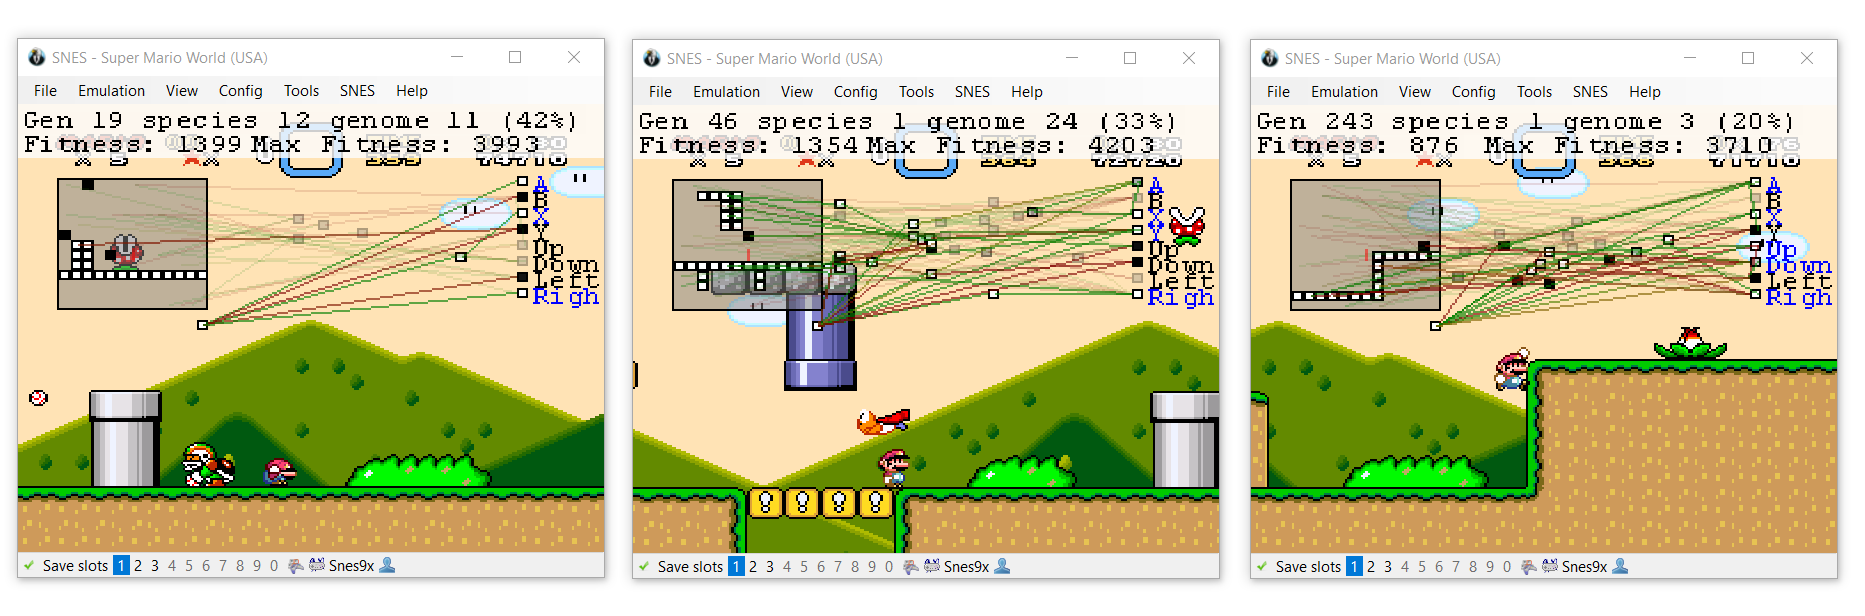
\includegraphics[width=1\textwidth]{graphics/mario/mario3}
			\caption{MarI/O simulation}
			\label{fig:mario}
		\end{figure}
		As mentioned in section \ref{sec:related:tools} MarI/O (see figure \ref{fig:mario}) is an implementation of \gls{neat}-algorithm written in \gls{lua}. It provides a solution for automatic learning of the game Super Mario World. In Super Mario World a level is a two-dimensional map with steady as well as moving obstacles.
		Some of them block the path to the goal and others cause damage to Mario's health. A few of them give health upgrades to Mario or add coins to the player's account, although the coins are ignored in the implementation of the \gls{ai}. Since there are many positions in which Mario can stay and the speed of the game depends mostly on the player and his/her/its decisions the environment of Super Mario World is rather complex when compared to the second game Flappy Bird \ref{sec:analysis:flappy}.\\
		This complex world leaves the expectation that many hundred thousand runs are necessary to learn how to complete a level. However, MarI/O implementation reached to goal after approximately $2664.29$ runs on average in the simulations described later in this section. Still, 2 of the 9 simulations didn't reach the goal once.\\
		\todo{fitness function, formlar? when was goal reached} \\
		Later in this section, 3 figures with 3 similar graphs will be shown. The three different figures display the success of the algorithm in different classes of initial population size. Since the \gls{neat}-algorithm used does not produce a deterministic amount of populations after the first generation (in general: Generation 0), the initial population size defines these classes. There were three classes chosen with a scaling factor of 5 between them. These initial population sizes are 10, 50 and 250. Whether or not the initial population sizes are well-chosen will be discussed shortly in the conclusion section (see \ref{sec:compare:params}) of this chapter. Depending on the evolution of the \gls{nn}, there are a certain amount of generations evolved. Every generation contains their own set of species. And on the other hand, the species contain the genomes. In generation 0 every species contains only one genome each. The sum of all genomes in all species of a generation is called the population. In the cases where the initial population size is 10 or 50 over time to many generations were created to show a viewable graph in the end. That's why only 30 generations were picked in the display with even distances between them. Still, a continuous line with the best run of a population is showed above all generations, even the skipped ones. \\
		In the later descriptions of the population classes, there are two types of runs introduced. First is the "plot-run" which indicates the simulation and the graph. Inside this graph, there were many "runs" which represent the runs of the population (genomes) of each species. In figure \ref{fig:mario} there are 3 individual runs displayed. On average one plot-run consists of $4217.\overline{2}$ runs, whereas population 10 has $2828$ runs on average, population 50 consists of $4494.\overline{6}$ runs on average and population 250 of $5329$ runs averaged.\\
		In order to understand the fundamental differences of these simulations, the population classes are examined in more detail: 
		\paragraph{Population 10 / Generation 500}
			\label{par:mario10}
			\begin{figure}[h]
				\centering
				\begin{minipage}{0.33\textwidth}
					\centering
					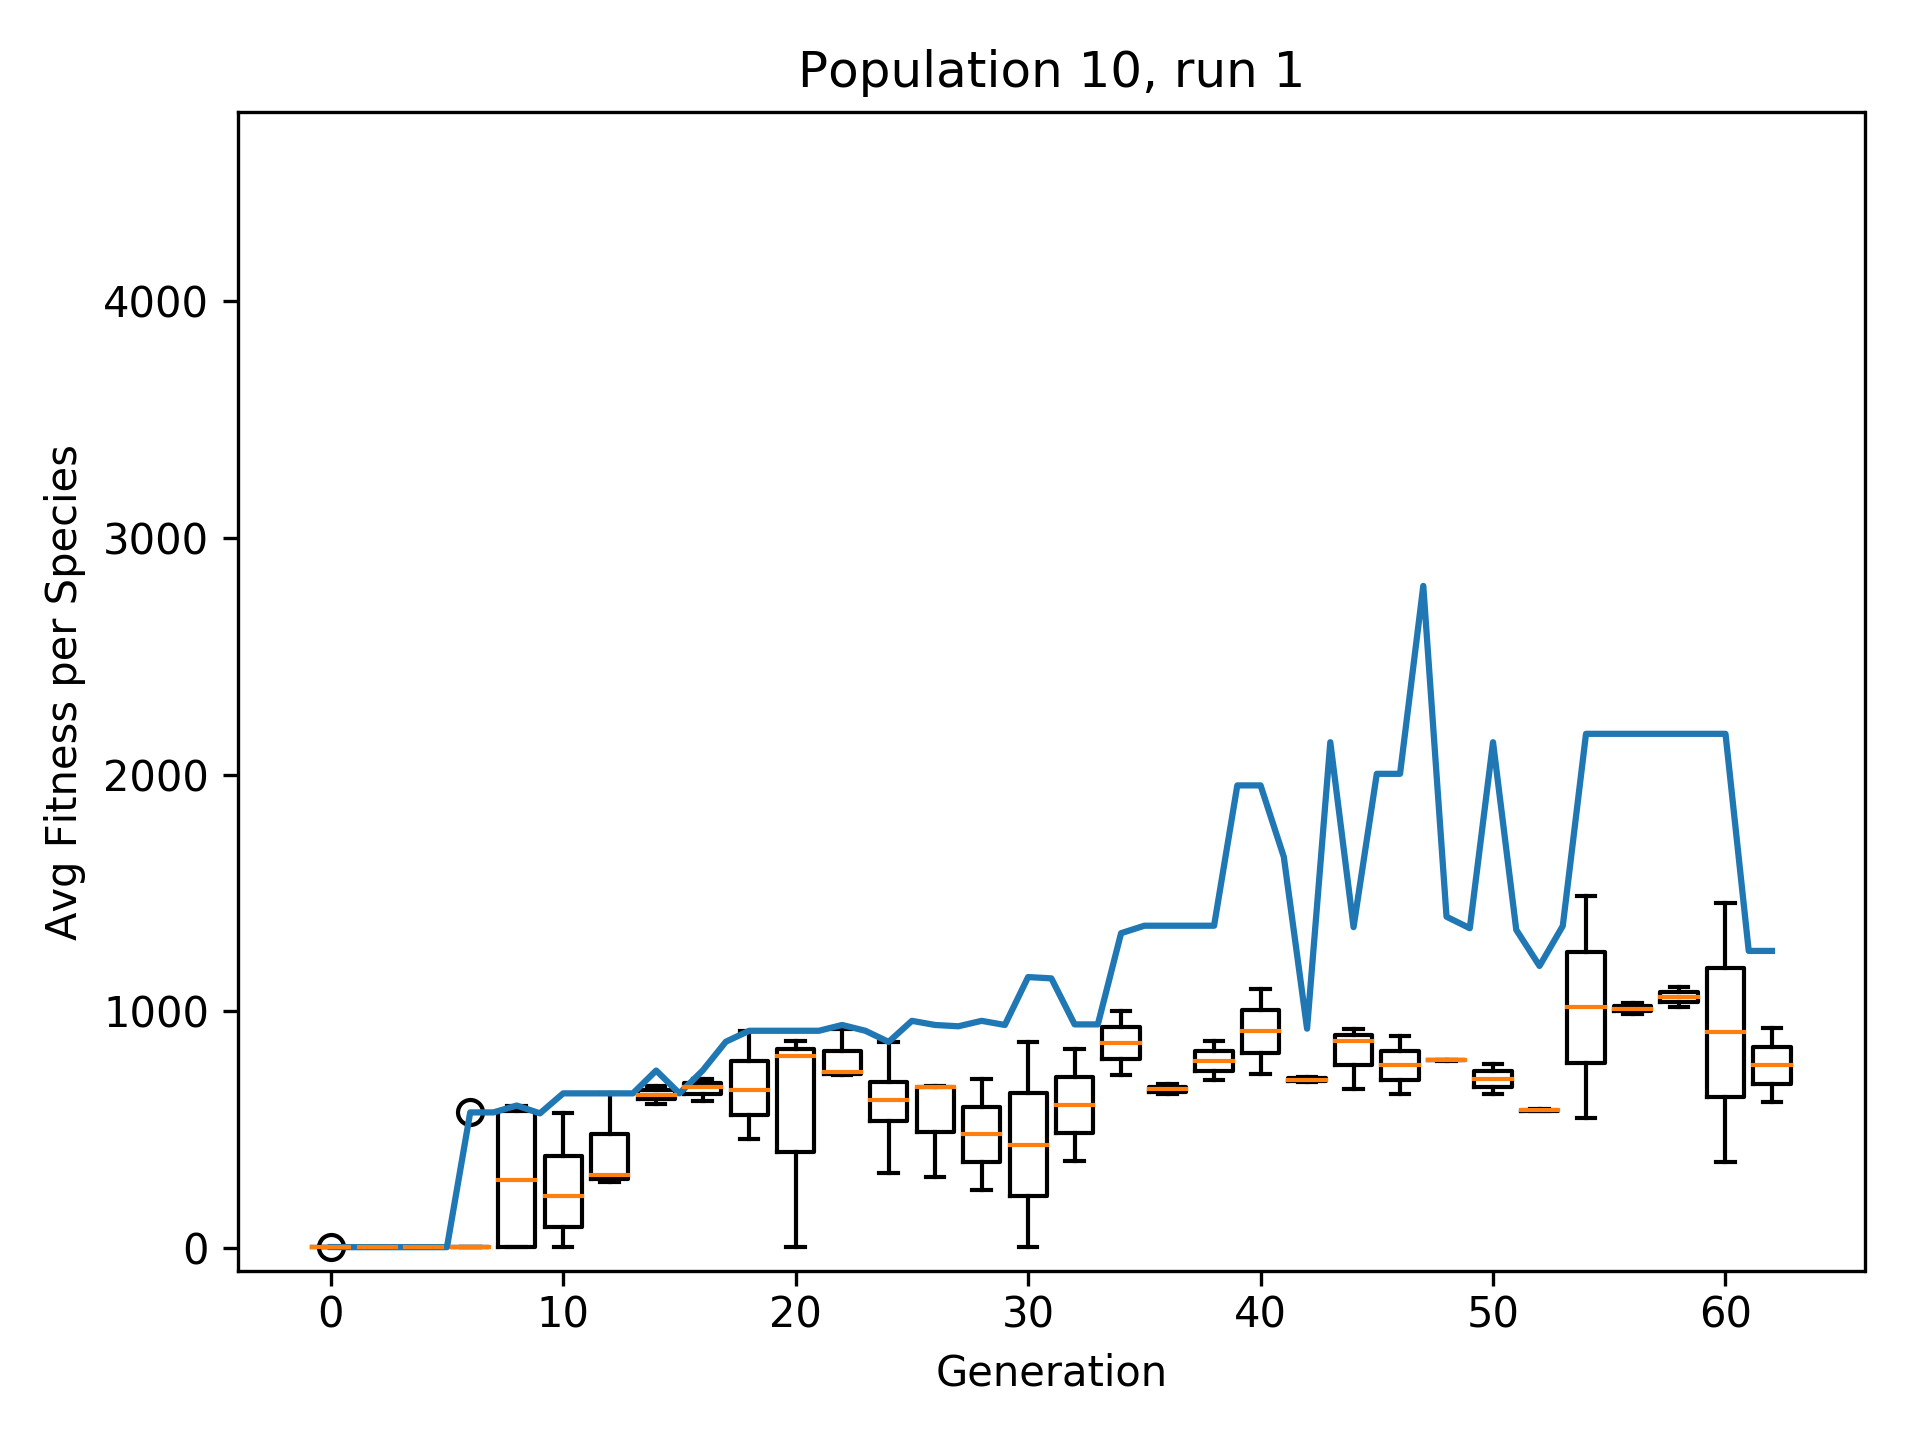
\includegraphics[width=1\textwidth]{graphics/mario/pop10_run1} % first figure itself
				\end{minipage}\hfill
				\begin{minipage}{0.33\textwidth}
					\centering
					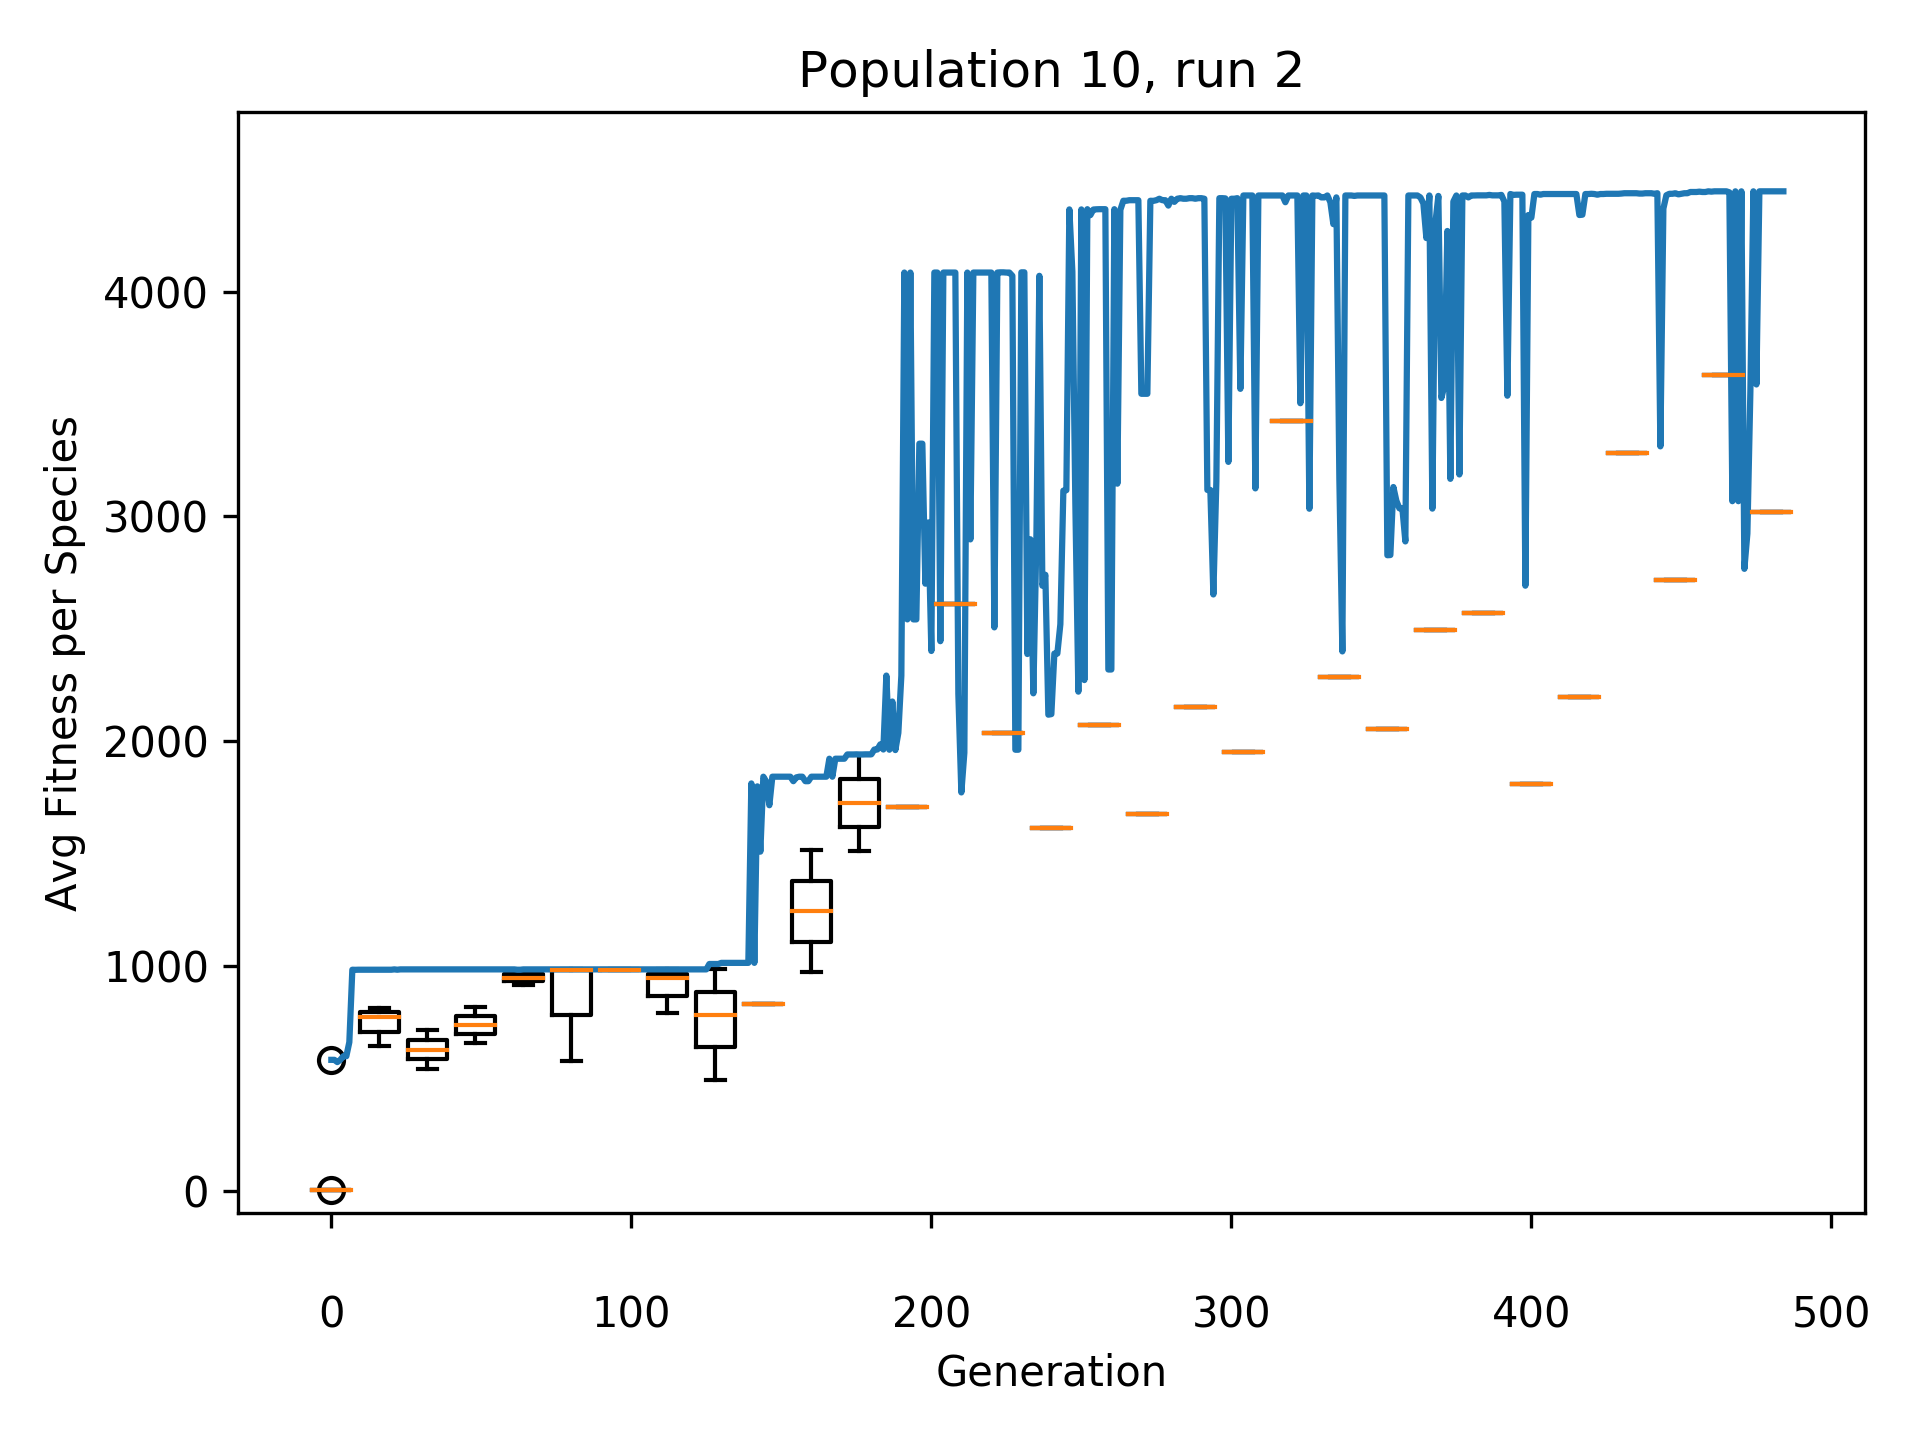
\includegraphics[width=1\textwidth]{graphics/mario/pop10_run2} % second figure itself
				\end{minipage}
				\begin{minipage}{0.33\textwidth}
					\centering
					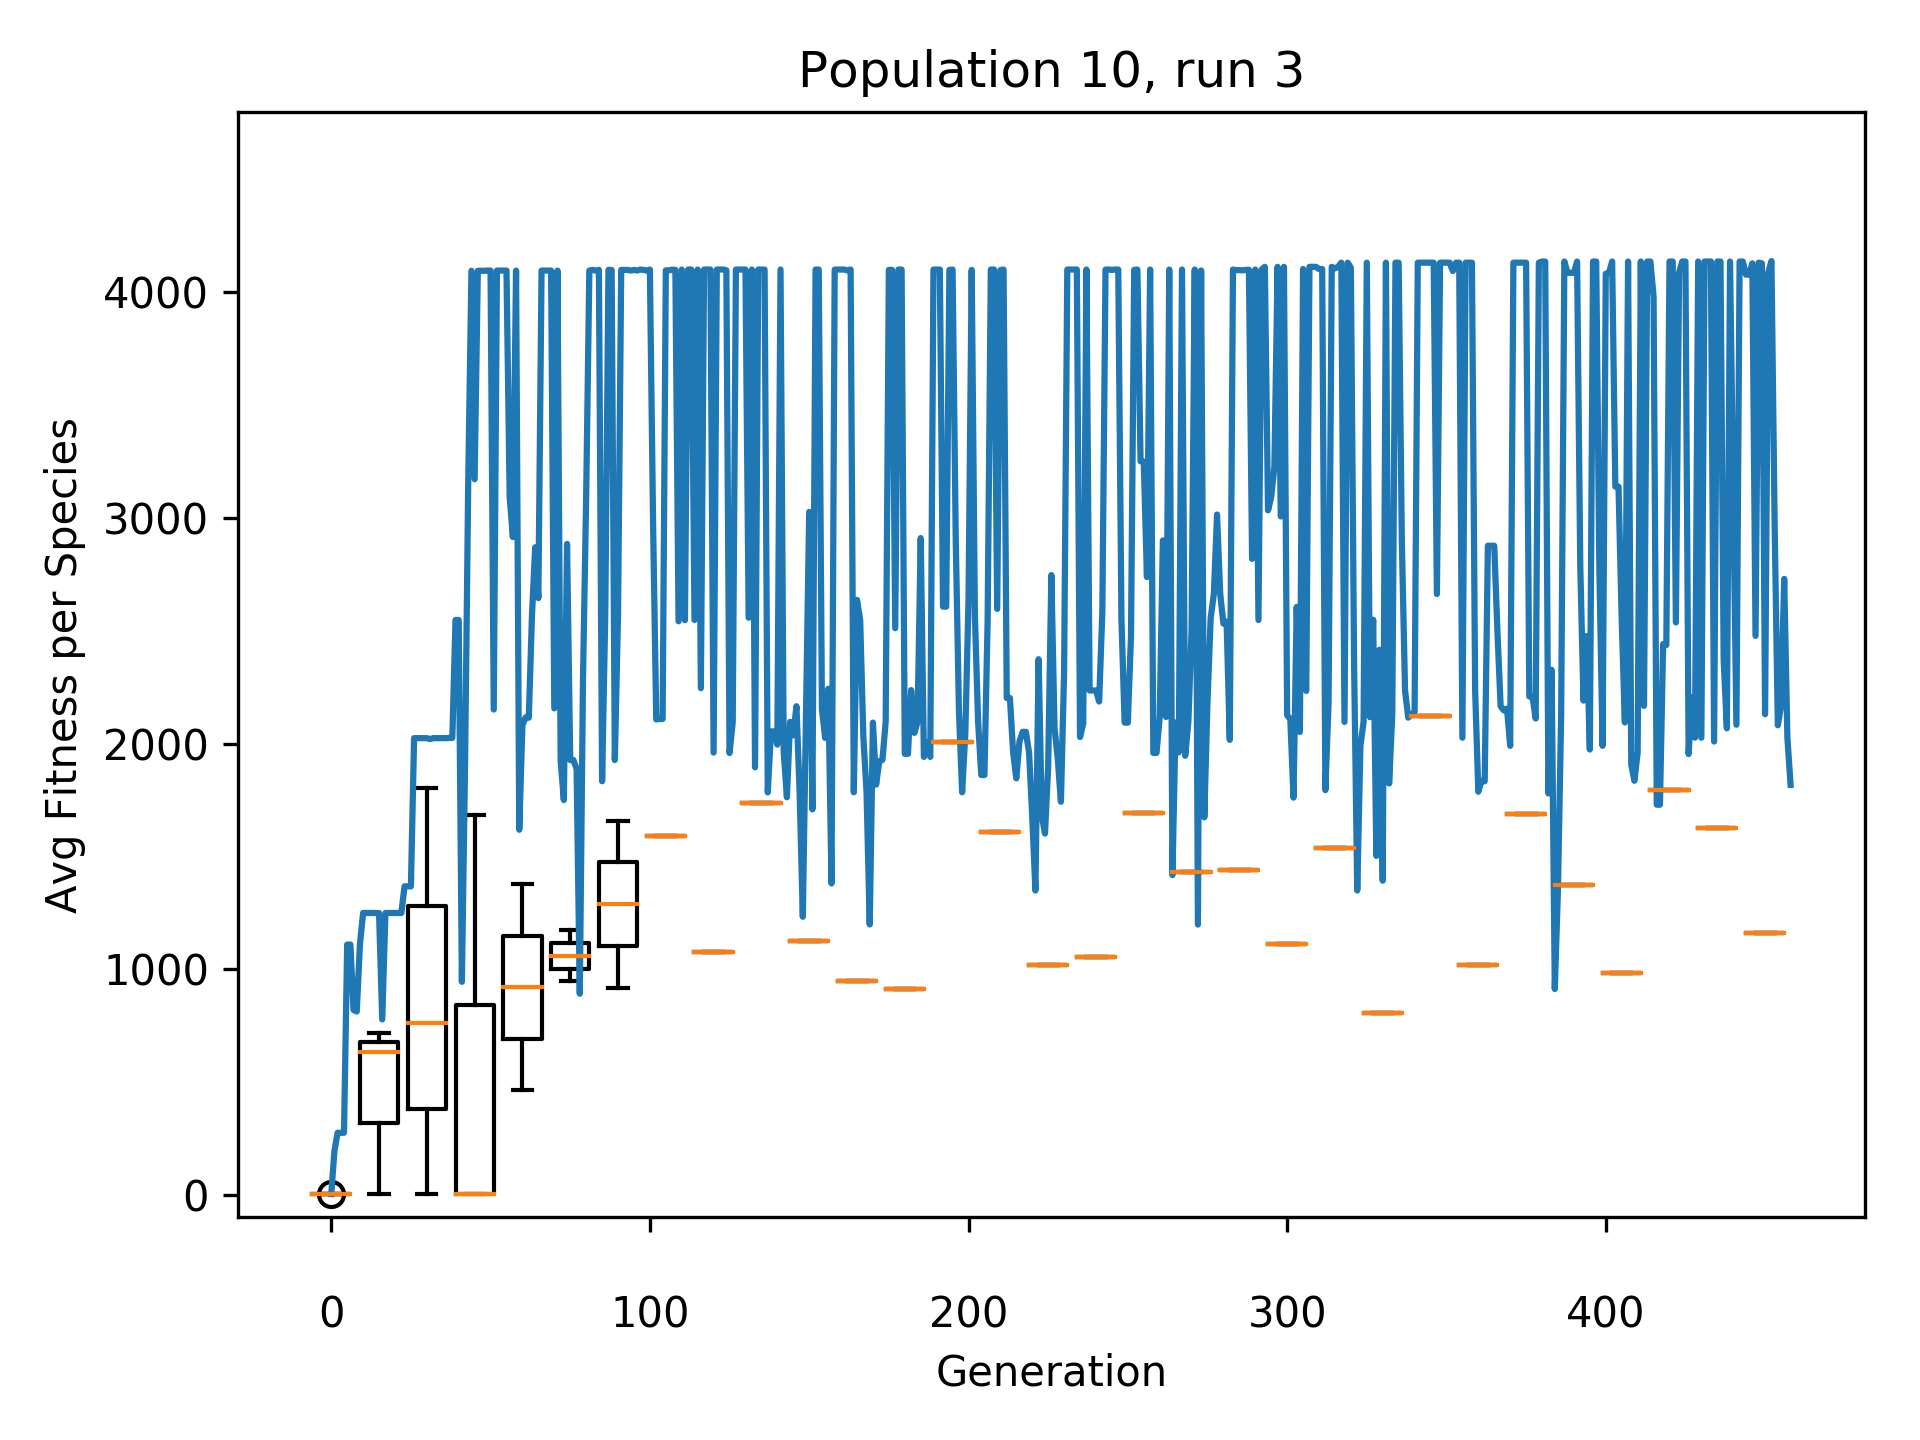
\includegraphics[width=1\textwidth]{graphics/mario/pop10_run3} % second figure itself
				\end{minipage}
				\caption{MarI/O Population 10}
				\label{fig:mario10}
			\end{figure}
			As it is visible in figure \ref{fig:mario10} the vertical axis shows the fitness score average of the genomes within a species. The horizontal axis portraits the generations containing the species. Each generation contains up to 10 populations which are divided into species and genomes within species. This species division was made based on the \gls{neat} algorithm described in section \ref{sec:related:neat}. The best run of the genomes grouped by each generation is marked with a blue line. Therefore the blue line indicates the best overall run within a generation. Since the boxplot portrays the species's average score of each generation and the blue line shows the best run per genome (population), the boxplot and the blue line rarely meet. Still, the average population score is closer to the best run than in the next two population variants (see later in this section population 50 \ref{par:mario50} and population 250 \ref{par:mario250}). This can be calculated by taking the median of the species fitness and subtracting that number from the best run of the genomes:
			$average\_distance = \frac{\sum\nolimits_{g_i \in generations} max(g_i.genomes) - median(g_i.species)}{|generations|}\approx1107$ whereas $g_i.genomes$ and $g_i.species$ are lists of the respective fitness. \\
			In the three plot-runs on average $334.\overline{6}$ generations were created, which results in a skipping of generations inside the graphics of around $11.1\overline{5}$ generations averaged, between two displayed generations. Unfortunately, the first run crashed after generation 60. Still, because of the long runtime of the simulation, the plot-run was kept. However, indicated by plot-run 2 and 3, the population growth started after this generation. As it can be seen in the 3rd plot-run of figure \ref{fig:mario10}, sometimes runs over 3000 fitness score could be achieved even after the 30th generation. In plot-run 2 the average fitness of the single species left tends to rise, however, more and longer plot-runs would be needed to test this hypothesis.\\
			In each generations, there are up to 10 populations.
			In the first generation (Gen 0) no mating was done. So in the first generation there were 10 species spawned with one genome each. In the 10th generation on average only $4.\overline{3}$ species where left. After generation 50 maximal 3 species where left in all runs and after generation 190 in plot-run 2 and after generation 91 in plot-run 3, respectively, only 1 species was left for mating. The mating results into the crossover of species.\\
			All runs except plot-run 1 reached the goal (the end of the level) multiple times which can be seen by the fitness score being over 4000. However, plot-run 3 reached the goal the earliest with runs over 4096 starting from generation 44. Still, there was the most overall regress made in plot-run 3. This can be calculated by adding the differences between the best runs of each generation if the difference was negative: $average\_regress = \frac{\sum\nolimits_{g_i \in generations} min(max(g_i.genomes) - max(g_{i-1}.genomes), 0)}{|generations|}\approx-348$ again whereas $g_i.genomes$ is a list of the fitness of each genome inside the generation. The regress of plot-run 1 was $-88.27$ approximately and of plot-run 2 was around $-109.98$.\\
			In plot-run 1 the $average\_fitness\_increase =  \frac{\sum\nolimits_{g_i \in generations} max(g_i.genomes) - max(g_{i-1}.genomes)}{|generations|}\approx19.87$ was the biggest of the three plot-runs since the first plot-run ended early and plot-run 3 had many drawbacks. The average fitness increase of plot-run 2 was around $7.97$ and of plot-run 3 was only $3.95$ approximately. Since it is only slightly possible to extend the maximum score above the score of 4000 and plot-run 1 has never reached this ranking, plot-run 1 pointed out to have the best score increase per round. Every successful round, whereas Mario reached the goal will only minimize the fitness increase when averaged with the generation count. In other words, for an infinitely large amount of generations the $average\_fitness\_increase$ is expected to converge to $0$ since the game has an end-state in contrast to the game Flappy Bird, as it can be seen in section \ref{sec:analysis:flappy}. In mathematical terms: $\lim\limits_{n \to \infty} average\_fitness\_increase(n) = 0$, whereas the $average\_fitness\_increase(n)$ is defined as the average fitness increase of a set of n generations.
		
		\paragraph{Population 50 / Generation 100}
			\label{par:mario50}
			\begin{figure}[h]
				\centering
				\begin{minipage}{0.33\textwidth}
					\centering
					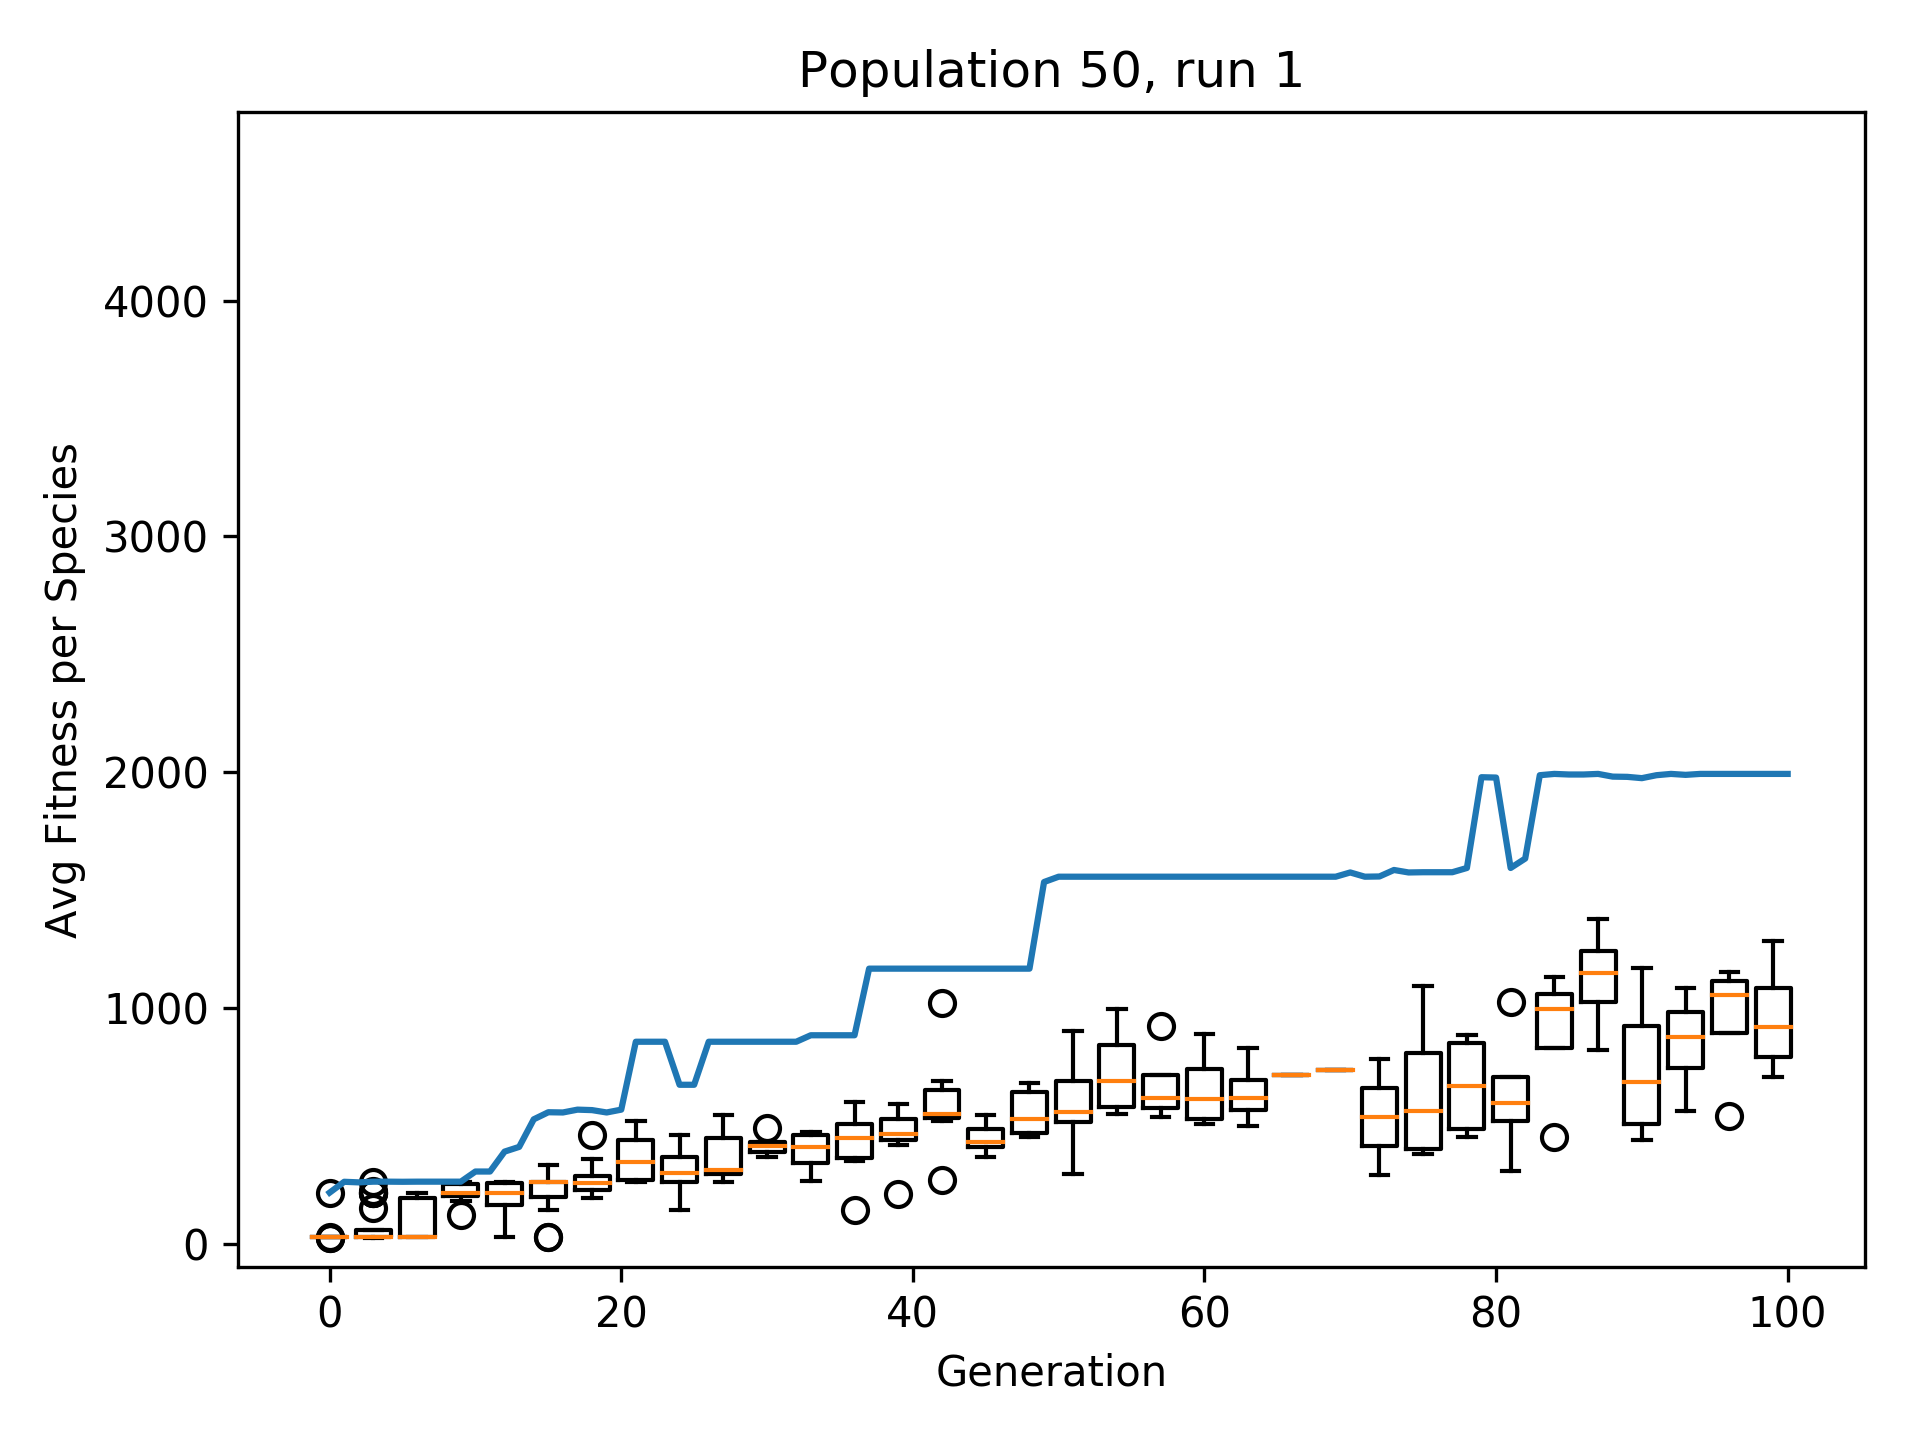
\includegraphics[width=1\textwidth]{graphics/mario/pop50_run1} % first figure itself
				\end{minipage}\hfill
				\begin{minipage}{0.33\textwidth}
					\centering
					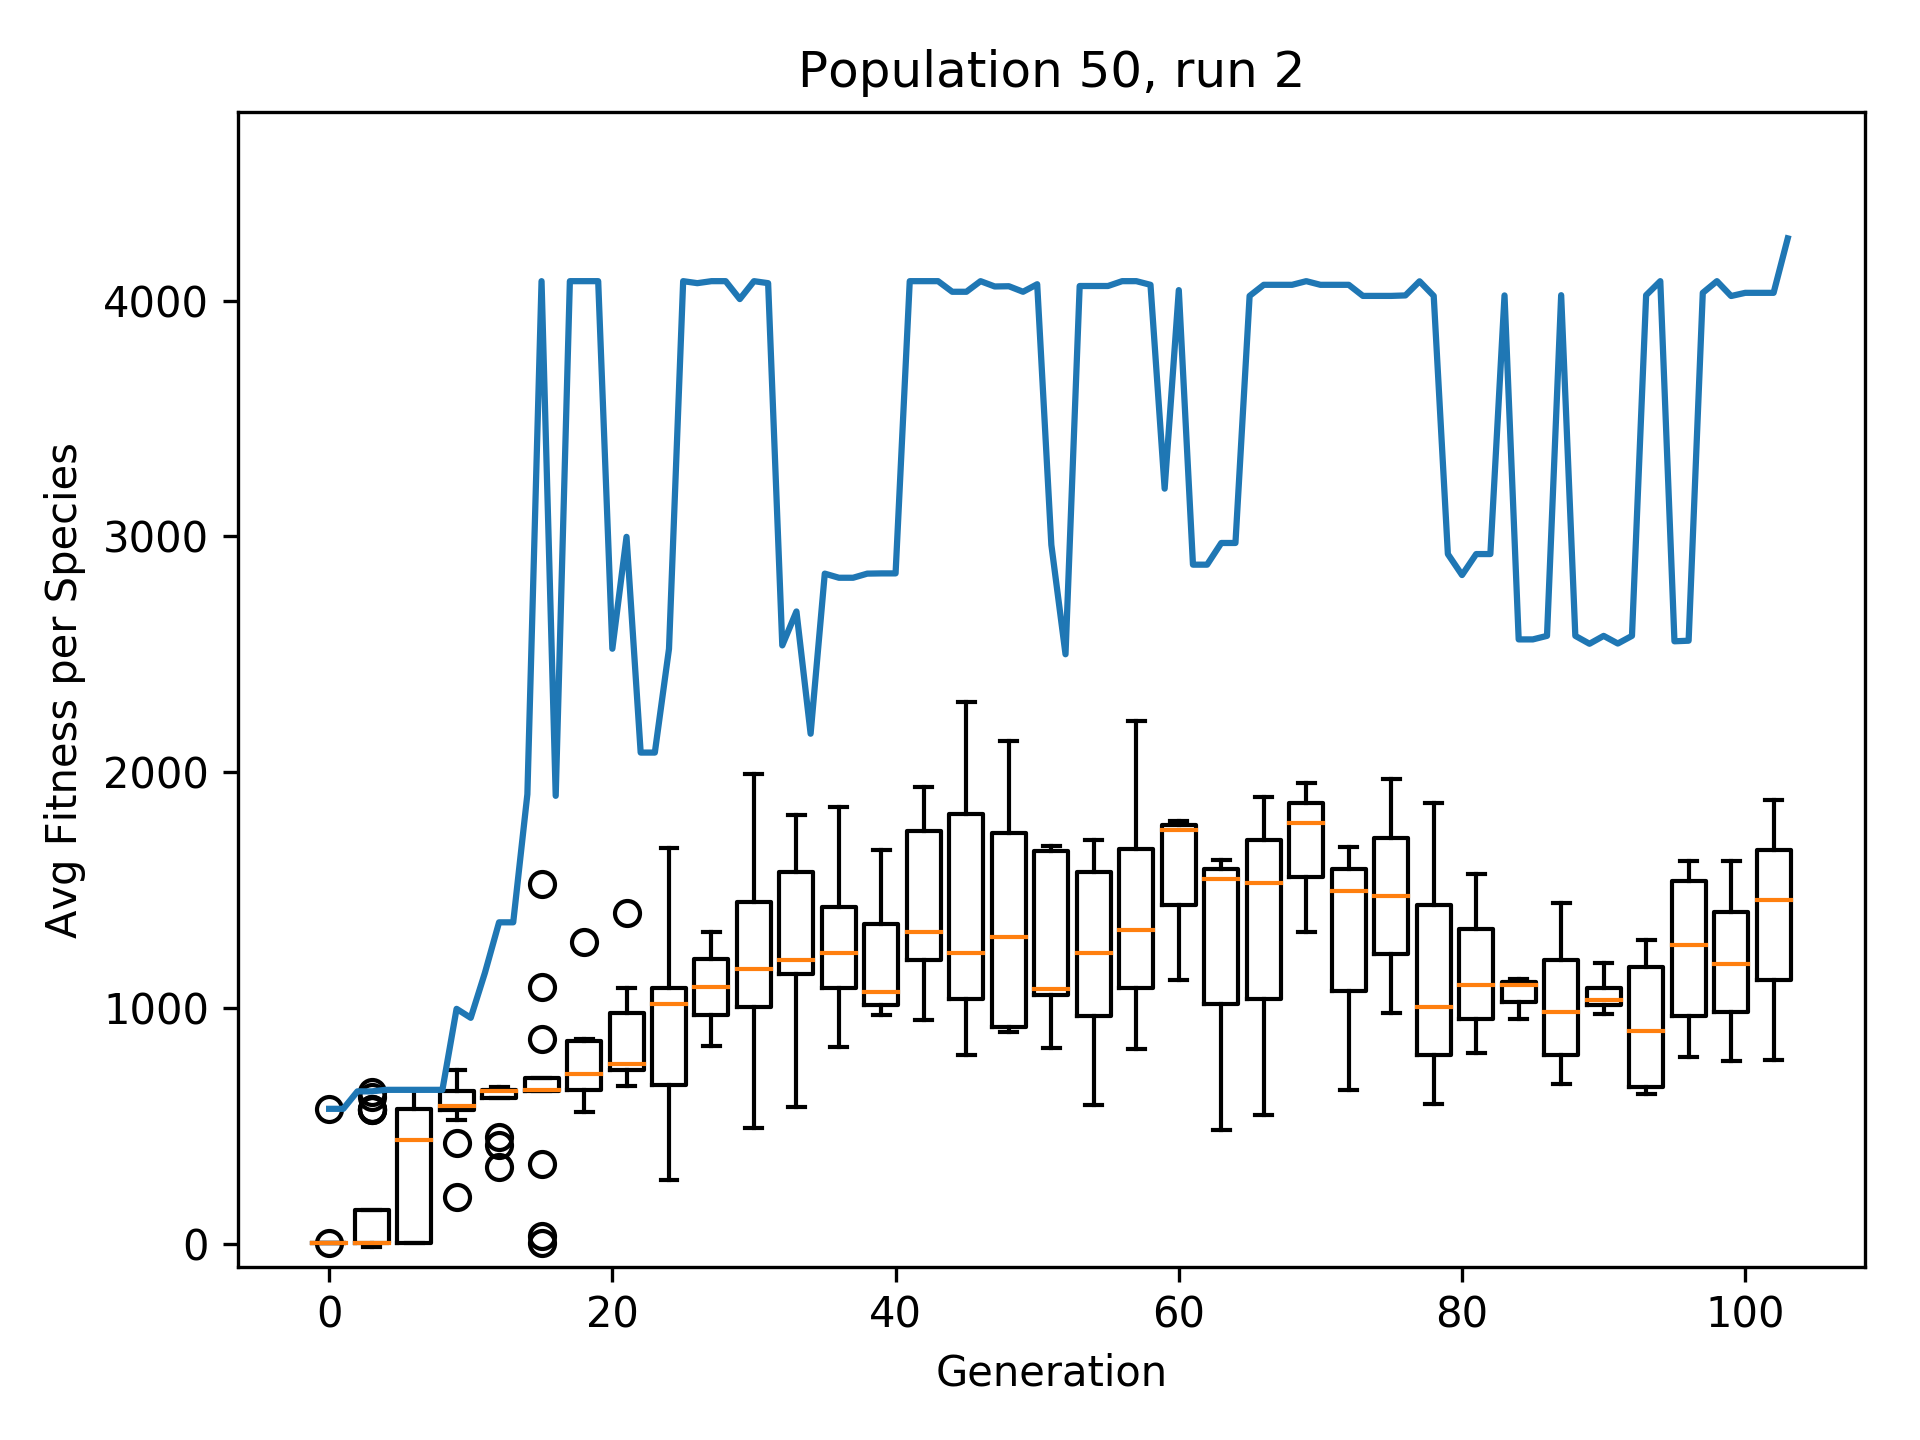
\includegraphics[width=1\textwidth]{graphics/mario/pop50_run2} % second figure itself
				\end{minipage}
				\begin{minipage}{0.33\textwidth}
					\centering
					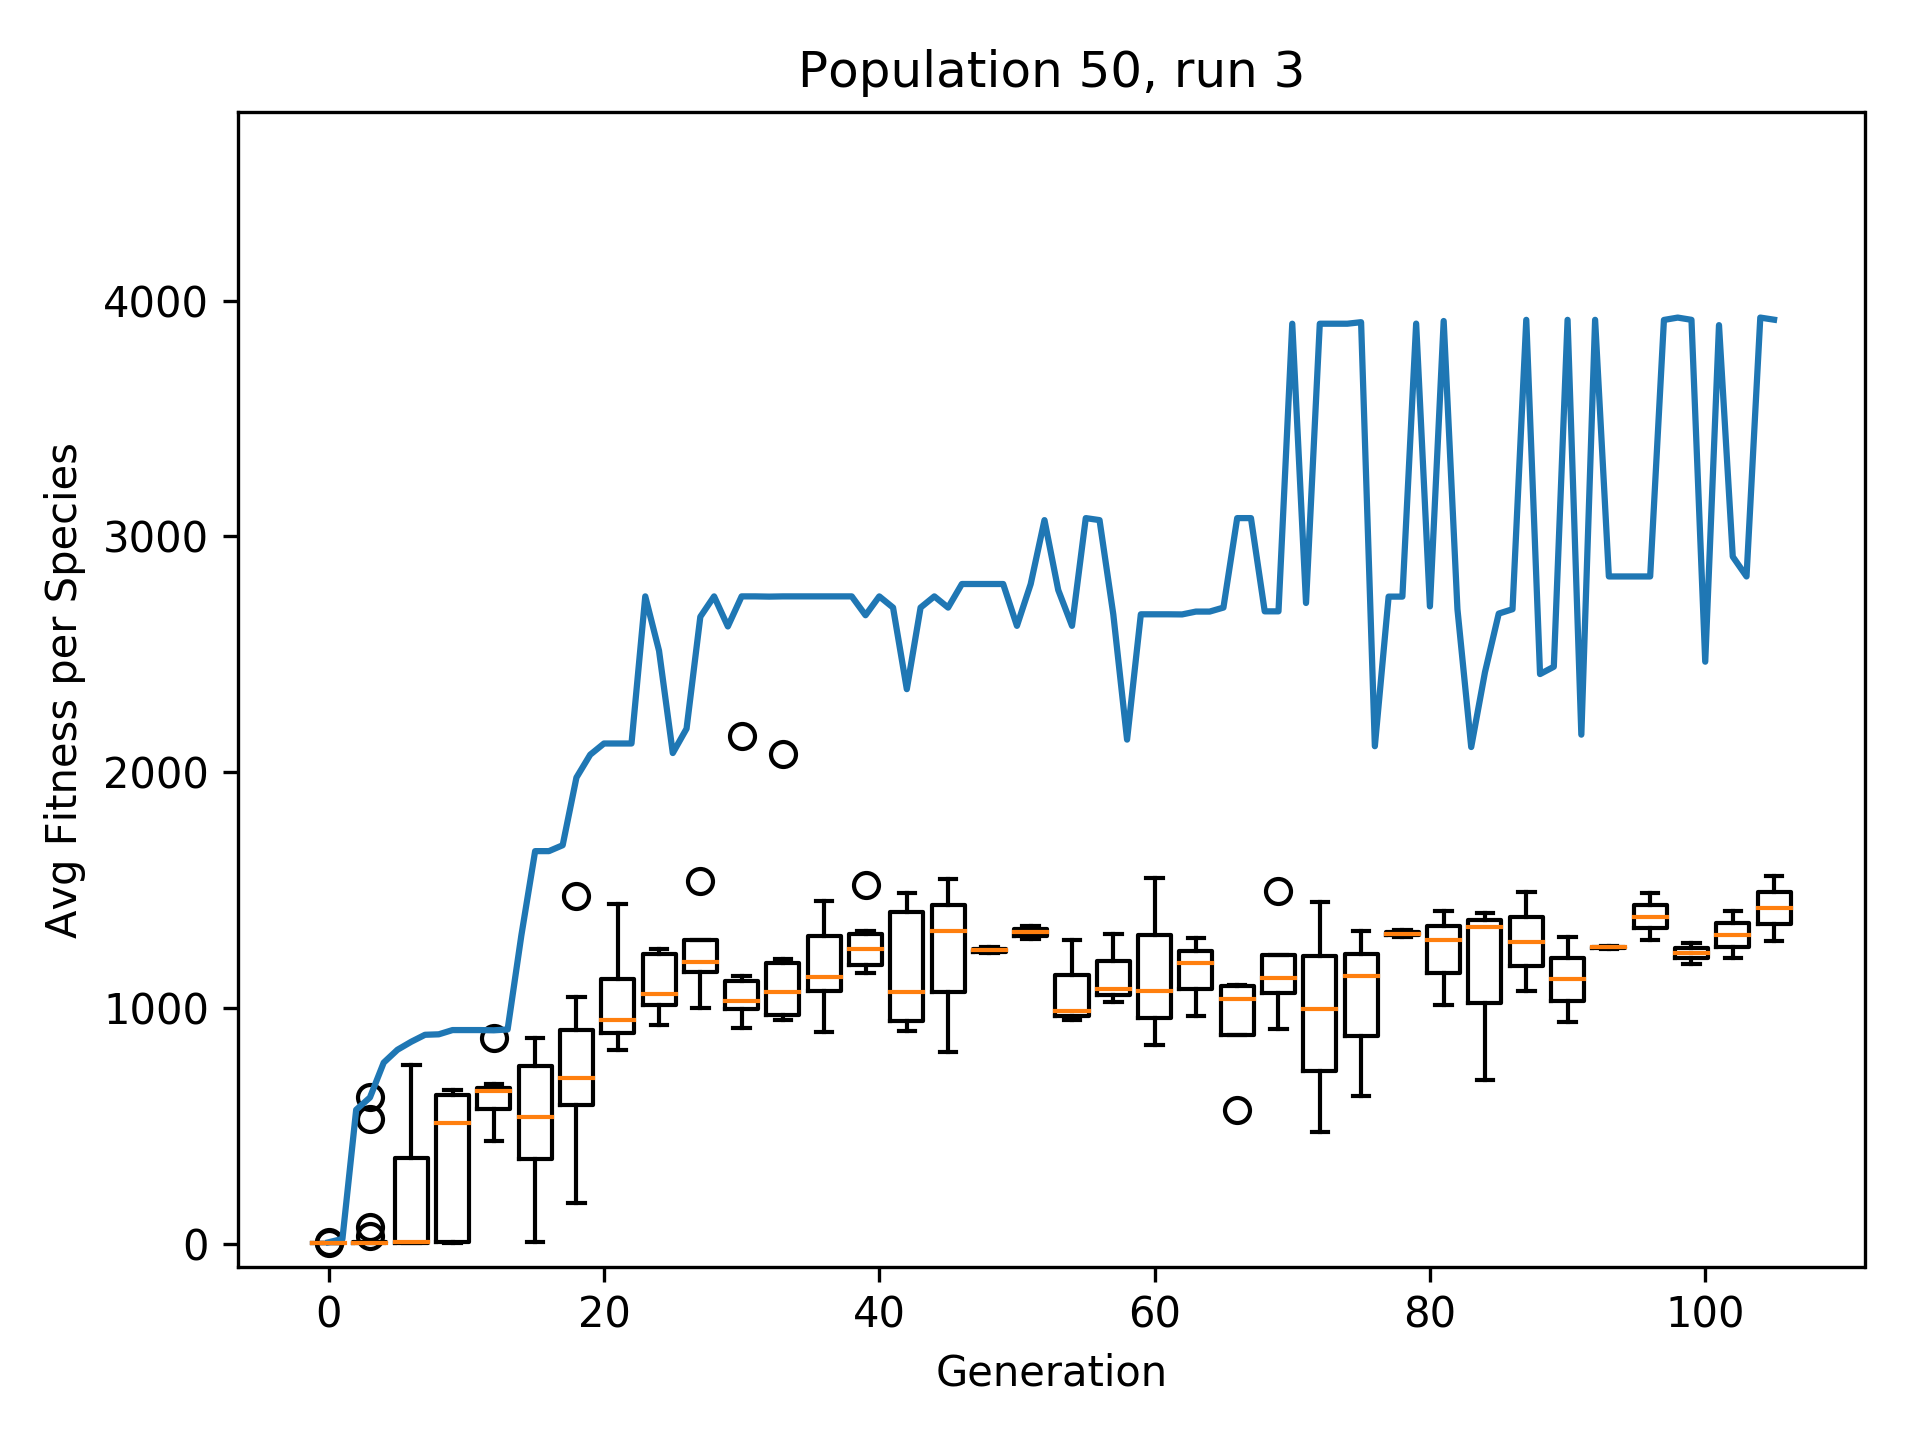
\includegraphics[width=1\textwidth]{graphics/mario/pop50_run3} % second figure itself
				\end{minipage}
				\caption{MarI/O Population 50}
				\label{fig:mario50}
			\end{figure}
			In this setup, the population count is up to 50, again distributed into species and genomes within species according to the MarI/O NEAT implementation. The $average\_distance$  between the median of the species of each generation to the best genome run of this generation is bigger than that of the simulation with its initial population size of 10 but it is smaller than in the last case. The $average\_distance$ was calculated as described in the previous simulation (population 10 \ref{par:mario10}) and the value is approximately $1406$.\\
			In this simulations the plot-runs where executed until there were over 100 generations (101 generations in plot-run 1, 104 in plot-run 2 and 106 in plot-run 3). This results in an average skipping of 3.456 generations between the display of two generations.\\
			In generation 0 there were 50 species spawned, again, with one genome each. In the 10th generation, there were 15 species left on average. At the end of generation 100, on average $3.\overline{3}$ species were left from the initial 50 generations.\\
			Interestingly the plot-run 1 couldn't learn to reach the goal. From this data, it is not trivial to predict if the breakthrough would have started within the next 50 generations or if this plot-run would have stayed low in its fitness score since there are no clear patterns to find in the graphical representation of these runs. In order to answer this question more profoundly, further and longer plot-runs have to be made and the big jumps between the fitness scores of each neighbor generation would have to be analyzed.\\
			Plot-run 2 and 3 had more luck in reaching the end, however, plot-run 3 had more stability in its high score results between generations. Still, after generation 70 plot-run 3 also shows stronger differences between its generation's high scores. Nevertheless, plot-run 2 reached the goal the earliest. The first time plot-run 2 achieved a fitness-score over 4000 was in generation 15 (it reached a score of $4082.5$), whereas plot-run 3 reached a maximum score of $3928$ in generation 98. Still, plot-un 3 reached to goal with a score of $3902$ the first time in generation 70. The 3rd plot-run has the highest $average\_fitness\_increase\approx36.92$ of the three plot-runs. Plot-run 1 has an $average\_fitness\_increase$ of $17.58$ approximately and plot-run 2 of $35.5$ precisely.\\
			Plot-run 2 and 3 have similar $average\_regress$ values with about $-158.02$ for plot-run 2 and $-152.37$ for plot-run 3. Because of the early end of a general low performance of plot-run 1, the $average\_regress$ is also the lowest with $-6.30$. Still, there were only 15 cases where the succeeding generation performed worse than the previews in plot-run 1 whereas there were 29 of these cases in plot-run 2 and 30 in plot-run 3. This indicated a certain stability in the first plot-run although the maximum score remained far lower than $3000$.
		
		
		\paragraph{Population 250 / Generation 30}
			\label{par:mario250}
			\begin{figure}[h]
				\centering
				\begin{minipage}{0.33\textwidth}
					\centering
					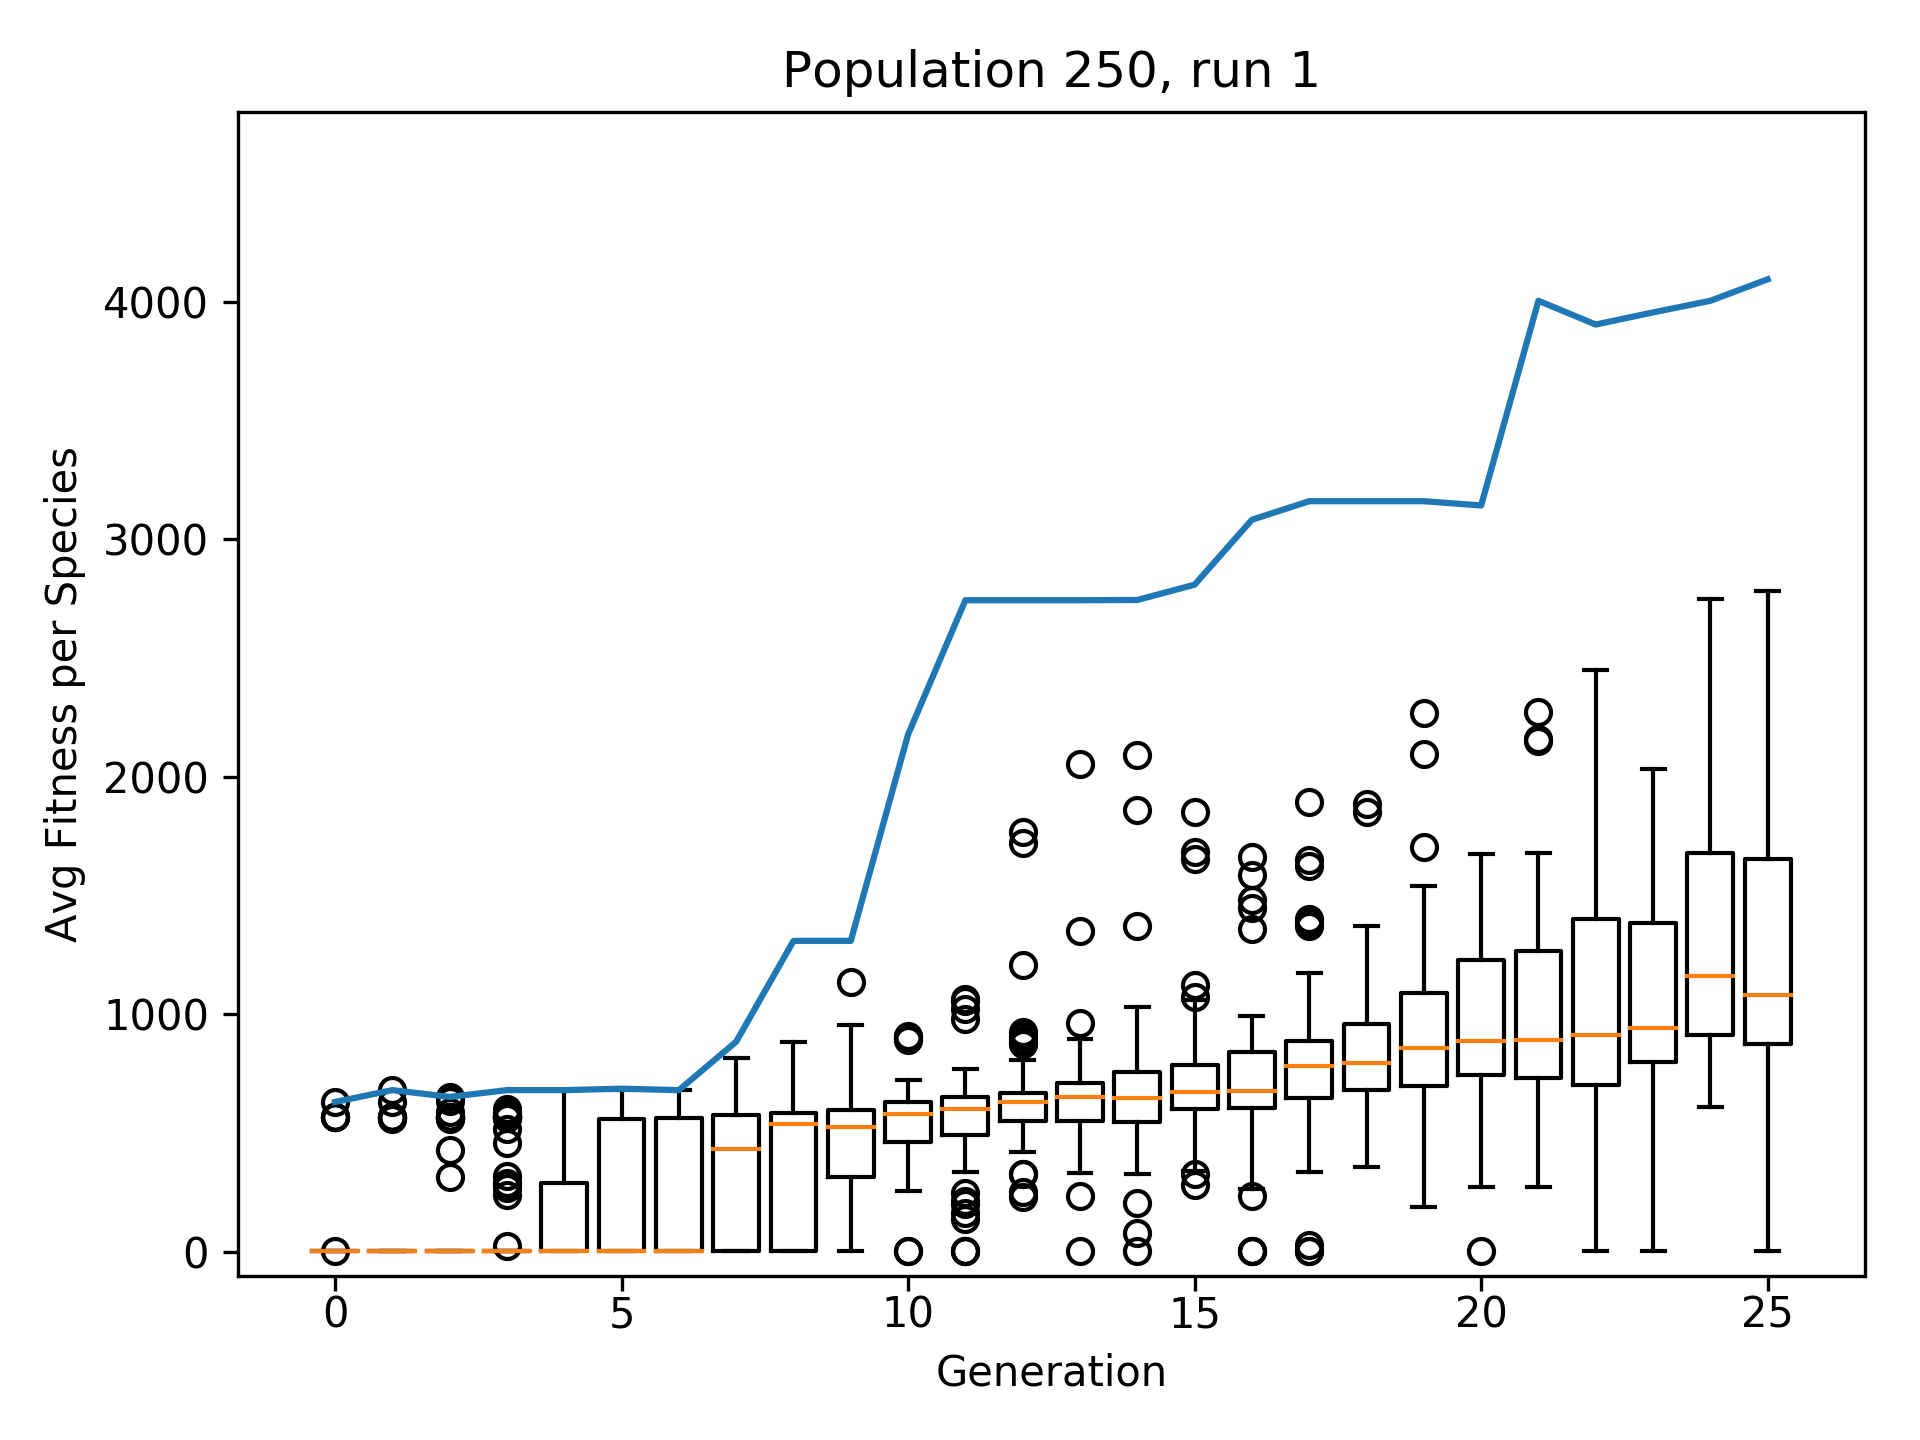
\includegraphics[width=1\textwidth]{graphics/mario/pop250_run1} % first figure itself
				\end{minipage}\hfill
				\begin{minipage}{0.33\textwidth}
					\centering
					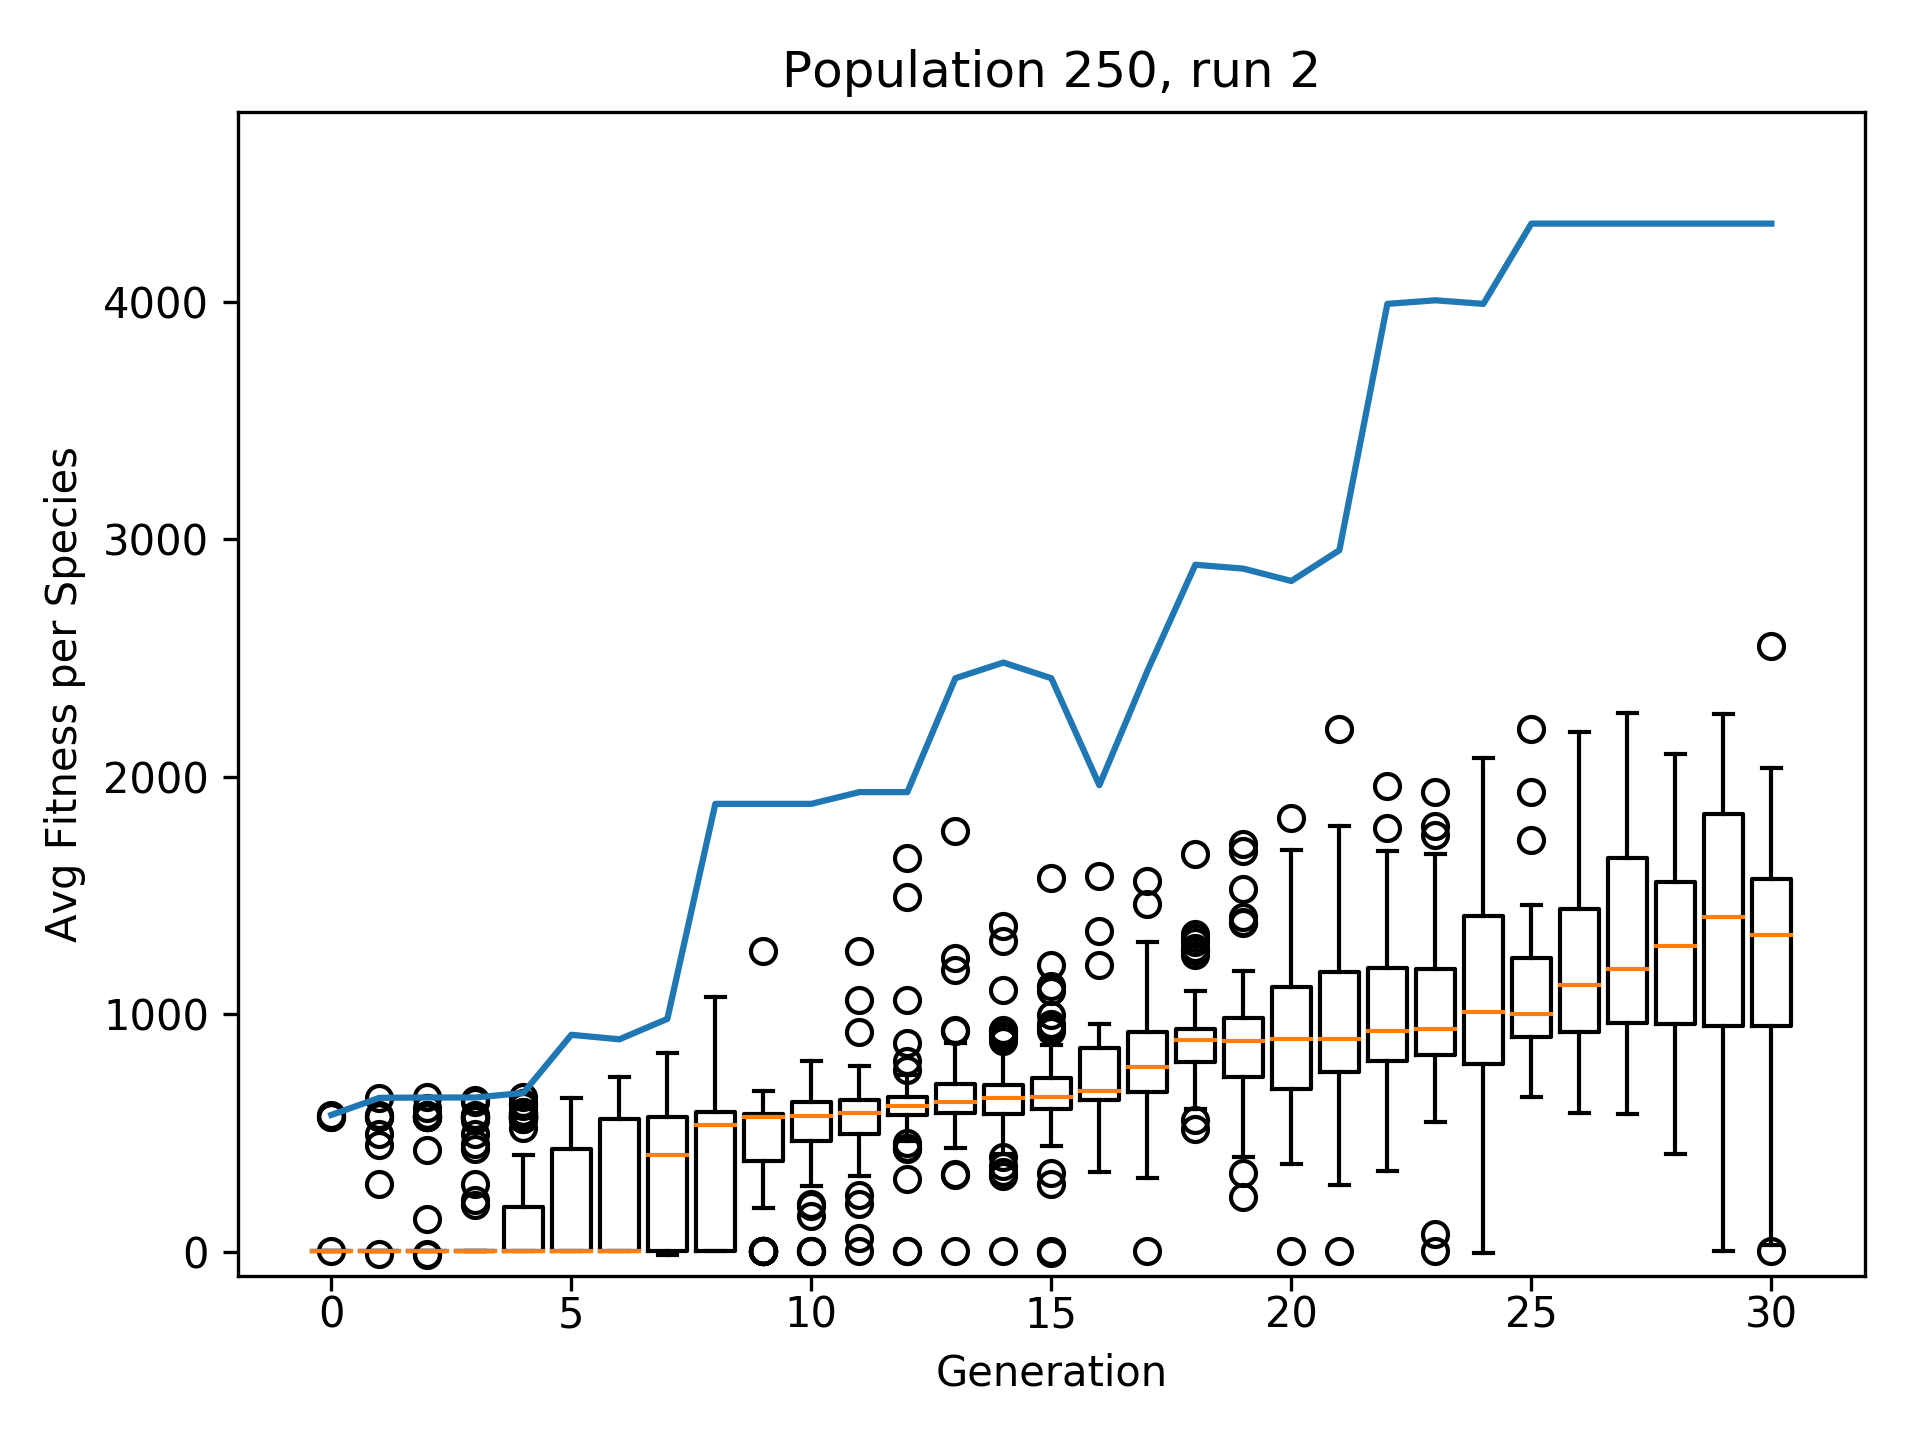
\includegraphics[width=1\textwidth]{graphics/mario/pop250_run2} % second figure itself
				\end{minipage}
				\begin{minipage}{0.33\textwidth}
					\centering
					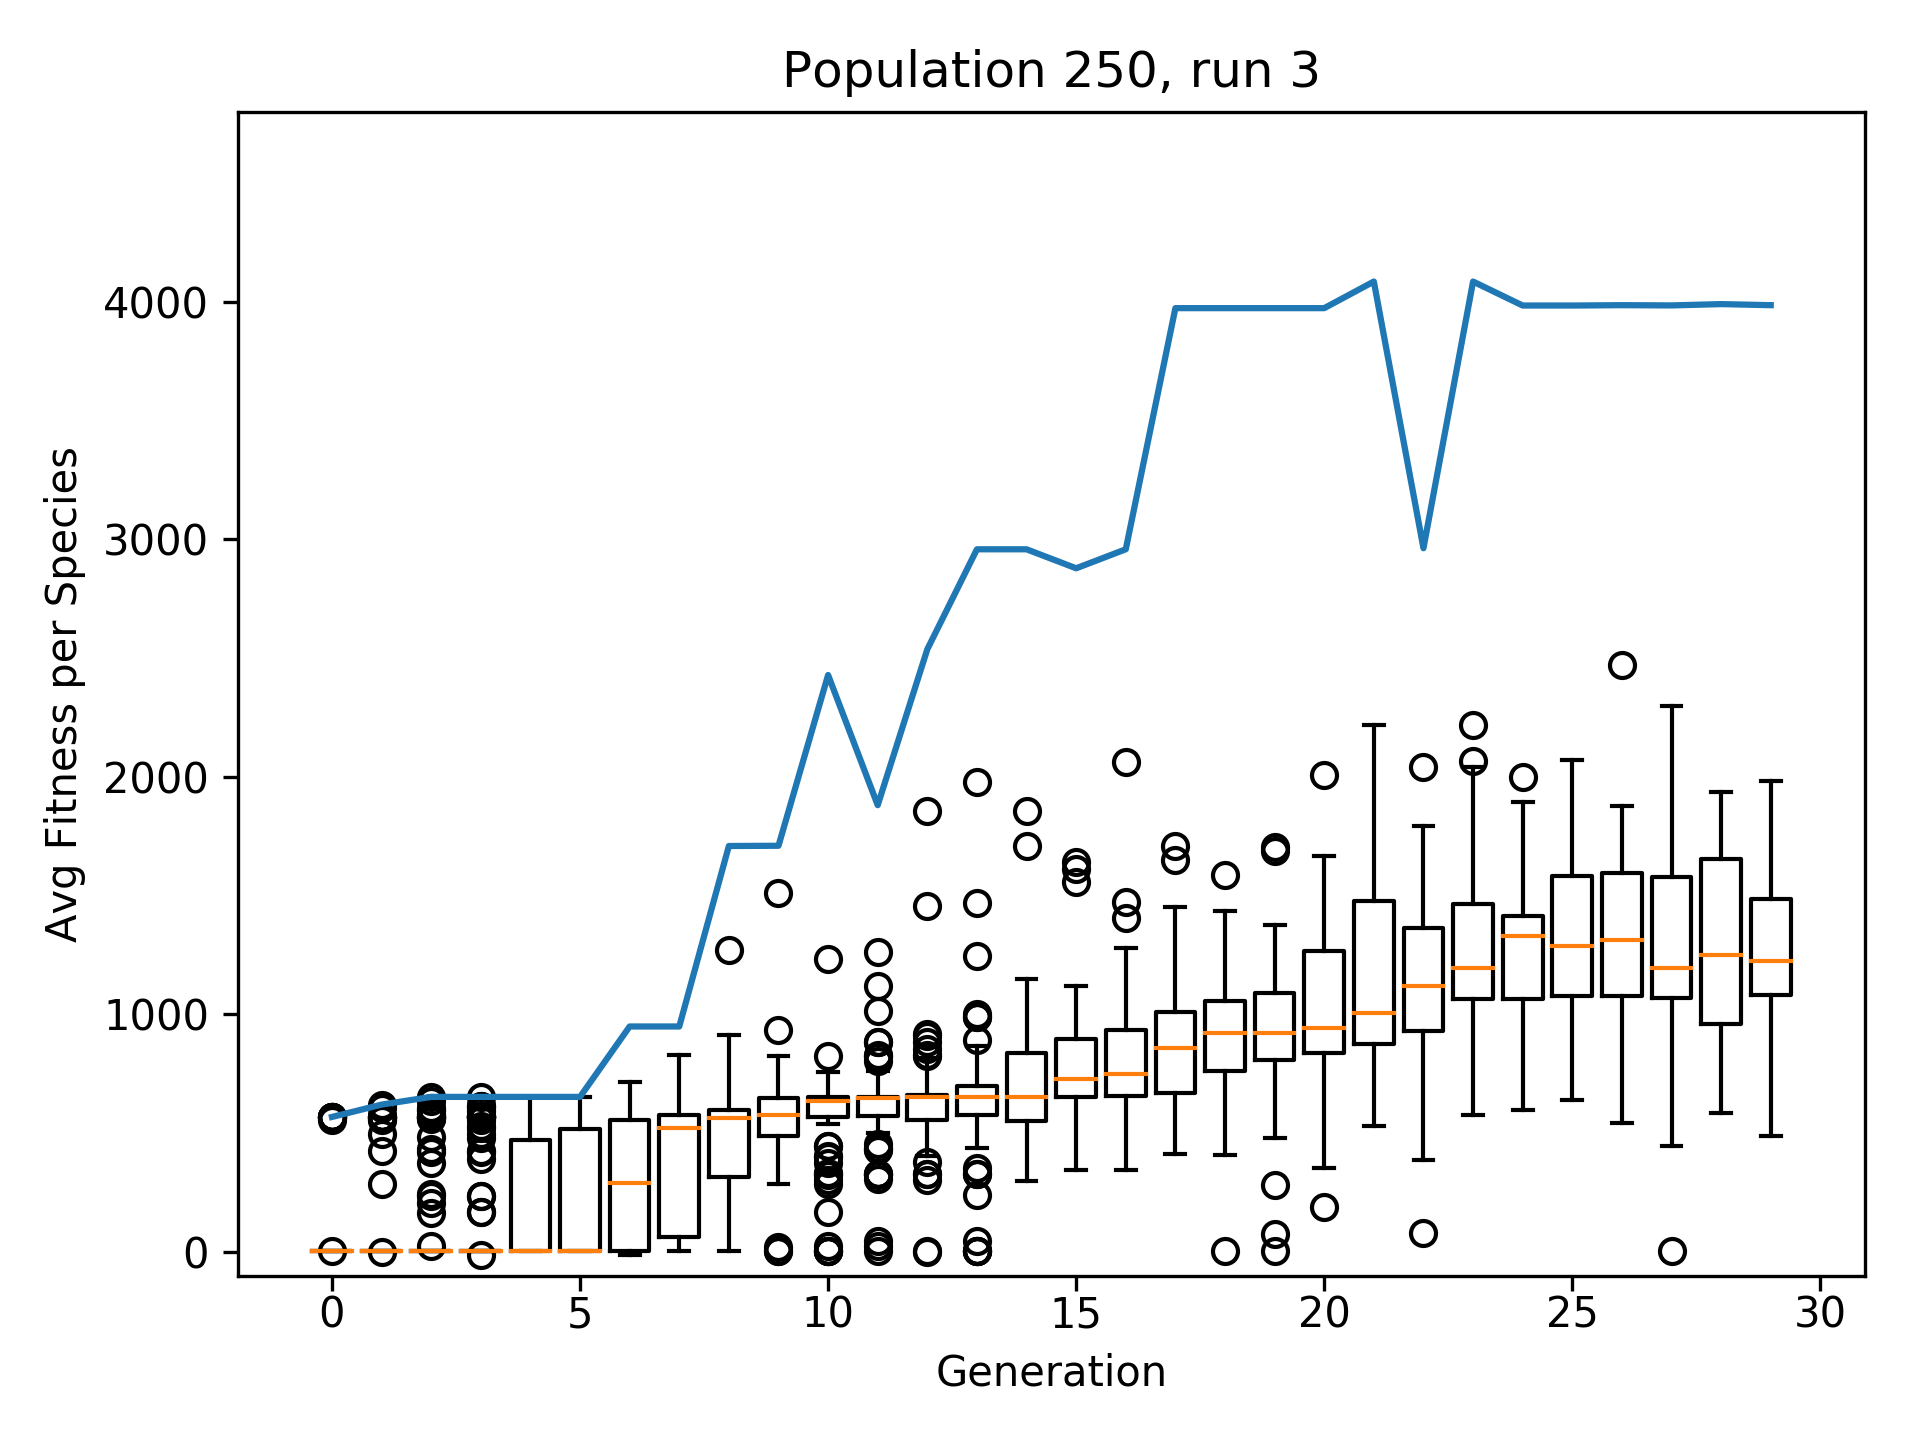
\includegraphics[width=1\textwidth]{graphics/mario/pop250_run3} % second figure itself
				\end{minipage}
				\caption{MarI/O Population 250}
				\label{fig:mario250}
			\end{figure}
			In figure \ref{fig:mario250} the population size is up to 250 in generation 0. In the first generation (Gen 0) 250 species are born with one genome each. The $average\_distance$ for this plot-runs is the biggest with approximately $1827$ when compared to the plot-runs with an initial population size of 10 and 50. In this plots, no generations had to be skipped in order to portray a descriptive graph since the maximum generation count is 30 in plot-run 2 (25 generations in run 1 and 29 generations in run 3).\\
			Already in the 6th generation, on average only 94.8 species were left. At the end of generation 25 there were 31 species left on average. \\
			Compared to the other two population classes, there are at least 7 times more species left at the end of the simulations which results in longer whiskers of the boxplot. The whiskers even contain bad starts with fitness-scores lower than 100 in plot-run 1 and 2. Interestingly the best runs are always exceptions after generation 6 (in plot-run 1 and 2 even earlier). \\
			Further, it is to mention that the plots are rather uniform compared to the plots of population 10 and 50. Therefore the $average\_fitness\_increase$ has similar values with a low variance which are $133.25$ for generation 1, around $121.08$ for generation 2 and $113.95$ for generation 3. The $average\_regress$ is the lowest in plot-run 1 at $-5.87$ approximately. This is because the maximum value of the succeeding generation is smaller than the previous generation in only 4 cases. The other two plot-runs have an $average\_regress$ of about $-19.97$ in plot-run 2 and $-61.92$ in plot-run 3. All of the plot-runs reached the end of the level even though plot-run 3 reached the end at generation 17, whereas plot-run 1 reached the end at generation 23 and plot-run 2 at generation 22.	
	
		\paragraph{Comparison of the results}
			\begin{table}[h]
				\centering
				\resizebox{\textwidth}{!}{
					\begin{tabular}[width=0.5\textwidth]{@{}ll|l|l|l|l@{}}
						\toprule
						{\Large MarI/O} & avg. runs /$\sigma$ 			& avg. fitness score /$\sigma$ 	& avg distance /$\sigma$ 	& avg. regress /$\sigma$ & avg. fitness increase /$\sigma$ 	\\ \midrule
						Population 10  	& 2828 /2055.44             	& 1231.42 /531.37      			& 1107.09 /534.5         	& -182.03 /144.01        & 10.6 /8.28             			\\
						Population 50  	& $4494.\overline{6}$ /176.09	& 960.96 /321.34       			& 1405.96 /664.75        	& -105.56 /86.01         & 30 /10.78              			\\
						Population 250 	& 5329 /656.74               	& 776.31 /57.88        			& 1826.32 /81.79        	& -29.25 /29.16          & 122.76 /9.76           			\\ \bottomrule
					\end{tabular}
				}
				\caption{MarI/O Population Comparison Overview}
				\label{tab:mario}
			\end{table}
			\todo{Differences and similarities between runs in graph} \\
			In order to compare the results, 5 distinct values (see table \ref{tab:mario}) of the plot-runs where calculated, as three of them were introduced in more detail earlier in this section \ref{par:mario10}. The first observations indicate that the average fitness score of each generation drops when establishing a bigger initial population. However, the standard deviation tends to drop as well. \\
			Also, the distance of the median of the species to the best run of the generation seems to become greater with a greater population count in generation 0. However, the average regress (if present) becomes lower with bigger population sizes and fewer generations, as well as it's deviation. Since there are fewer generations in the simulations with an initial population of 250 and these simulations having similar achievements, the average fitness increase is higher than in the other two simulation classes. The standard deviation of the average fitness increase is relatively similar.\\
			It is interesting to see how the fitness increase compares to the average distance value. Even though the fitness increase of population class 250 is higher than the fitness increase of population class 10, the distance remains large which indicates that the majority of runs stayed low and the average score of population class 10 is higher than in the other two population classes. Still, the other two classes remained more stable when taking the average regress into account. \\
			Another interesting point of view is the reaching of the end of the level (the goal). In all population classes, the goal was reached even though population class 1 and 2 didn't reach the goal in one plot-run each. Population 10 reached the goal in the first $24.48\%$ on average, only including the cases where the goal was reached. Population 50 reached the goal in the first $40,24\%$ on average and population class 250 in the first $69,47\%$.\\
			To summarize the results roughly it can be said that an initial population size of 10 promises faster and better results in a complex environment like Super Mario World, however, more stability can be reached when increasing the initial population size.
		
	% FLAPPY BIRD ###############################################################
	
	\section{NEAT\_FlappyBird}
		\label{sec:analysis:flappy}
		
		\begin{figure}[h]
			\centering
			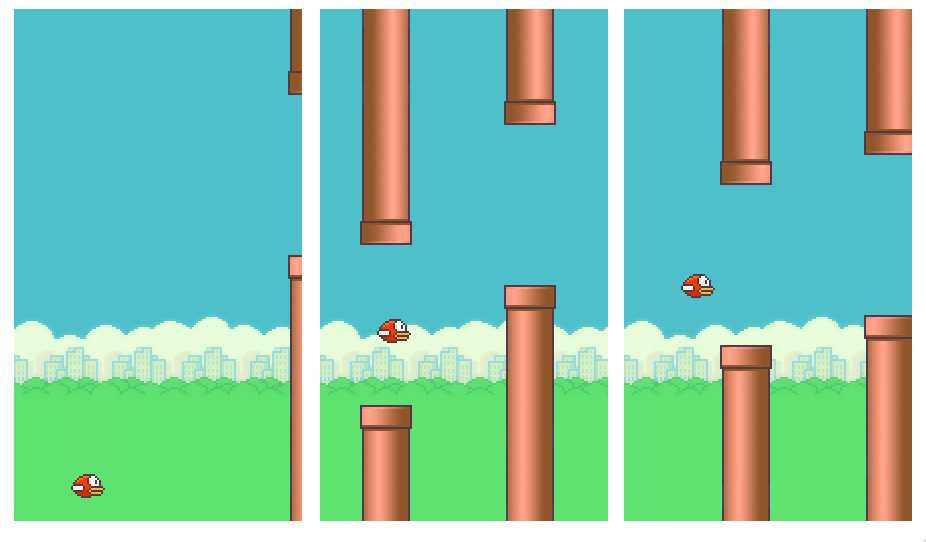
\includegraphics[width=1\textwidth]{graphics/flappy/flappy}
			\caption{Flappy Birds simulation}
			\label{fig:flappy}
		\end{figure}
	
		As mentioned in section \ref{sec:related:tools}, NEAT\_FlappyBird (see figure \ref{fig:flappy}) is an implementation of \gls{neat}-algorithm written in Python using the \gls{neat} framework NEAT-Python \footnote{\url{https://neat-python.readthedocs.io}, last accessed 30th October 2018}. It provides a solution for mastering the game Flappy Bird which was also rewritten in Python. In Flappy Bird, a level is a two-dimensional, infinite map with obstacles along the way. The player, in the representation of a bird, moves at a constant speed to the right, where new obstacles are generated. These obstacles are pipes which create gaps, through which the bird has to fly (see figur\ref{fig:flappy}). \\
		Therefore the player has only one input, namely if he/she/it wants to fly up, or if not then the player automatically falls down. Since there is only one decision to make the game is rather simple compared to Super Mario World (see section \ref{sec:analysis:mario}).\\
		\todo{fitnessfunction, formlar?}
		This simple set-up creates the expectation that the \gls{neat} algorithm should be able to find a solution with a score above a certain threshold (which is defined later in this section). In fact, all simulations exceeded this threshold and the generations used where far lower the maximum generation defined for this simulations. NEAT\_FlappyBird reached the fitness threshold after $1047.\overline{4}$ runs on average. \\
		In this section, 3 figures similar to the ones used in section \ref{sec:analysis:mario} are shown. However, this time these figures are split into two ranges since the details of the graph are too far apart. Therefore a simulation of a population class contains 3 plot-runs whereas one plot-run is displayed in 2 graphs of different ranges.  For the size of the population classes, the same 3 sizes were chosen as used in the MarI/O simulation, which are 10, 50 and 250. \\
		Again a maximum amount of 30 generations are displayed in the graphs when the generation size was bigger than 30. Luckily, this was only the case in the population 10 simulations. Also, again, the generations contain the species, which by themselves contain the genomes (the population). 
		As in MarI/O a "plot-run" indicates the simulation and the graph which was plotted based on the simulation. Inside this graph, there were many "runs" executed which represent the runs of the population (genomes) of each species. \\
		Now the simulations are examined in more detailed categorized by their population size:
		
		\paragraph{Population 10 / Generation 500}
			\begin{figure}[h!]
				\centering
				\begin{minipage}{0.33\textwidth}
					\centering
					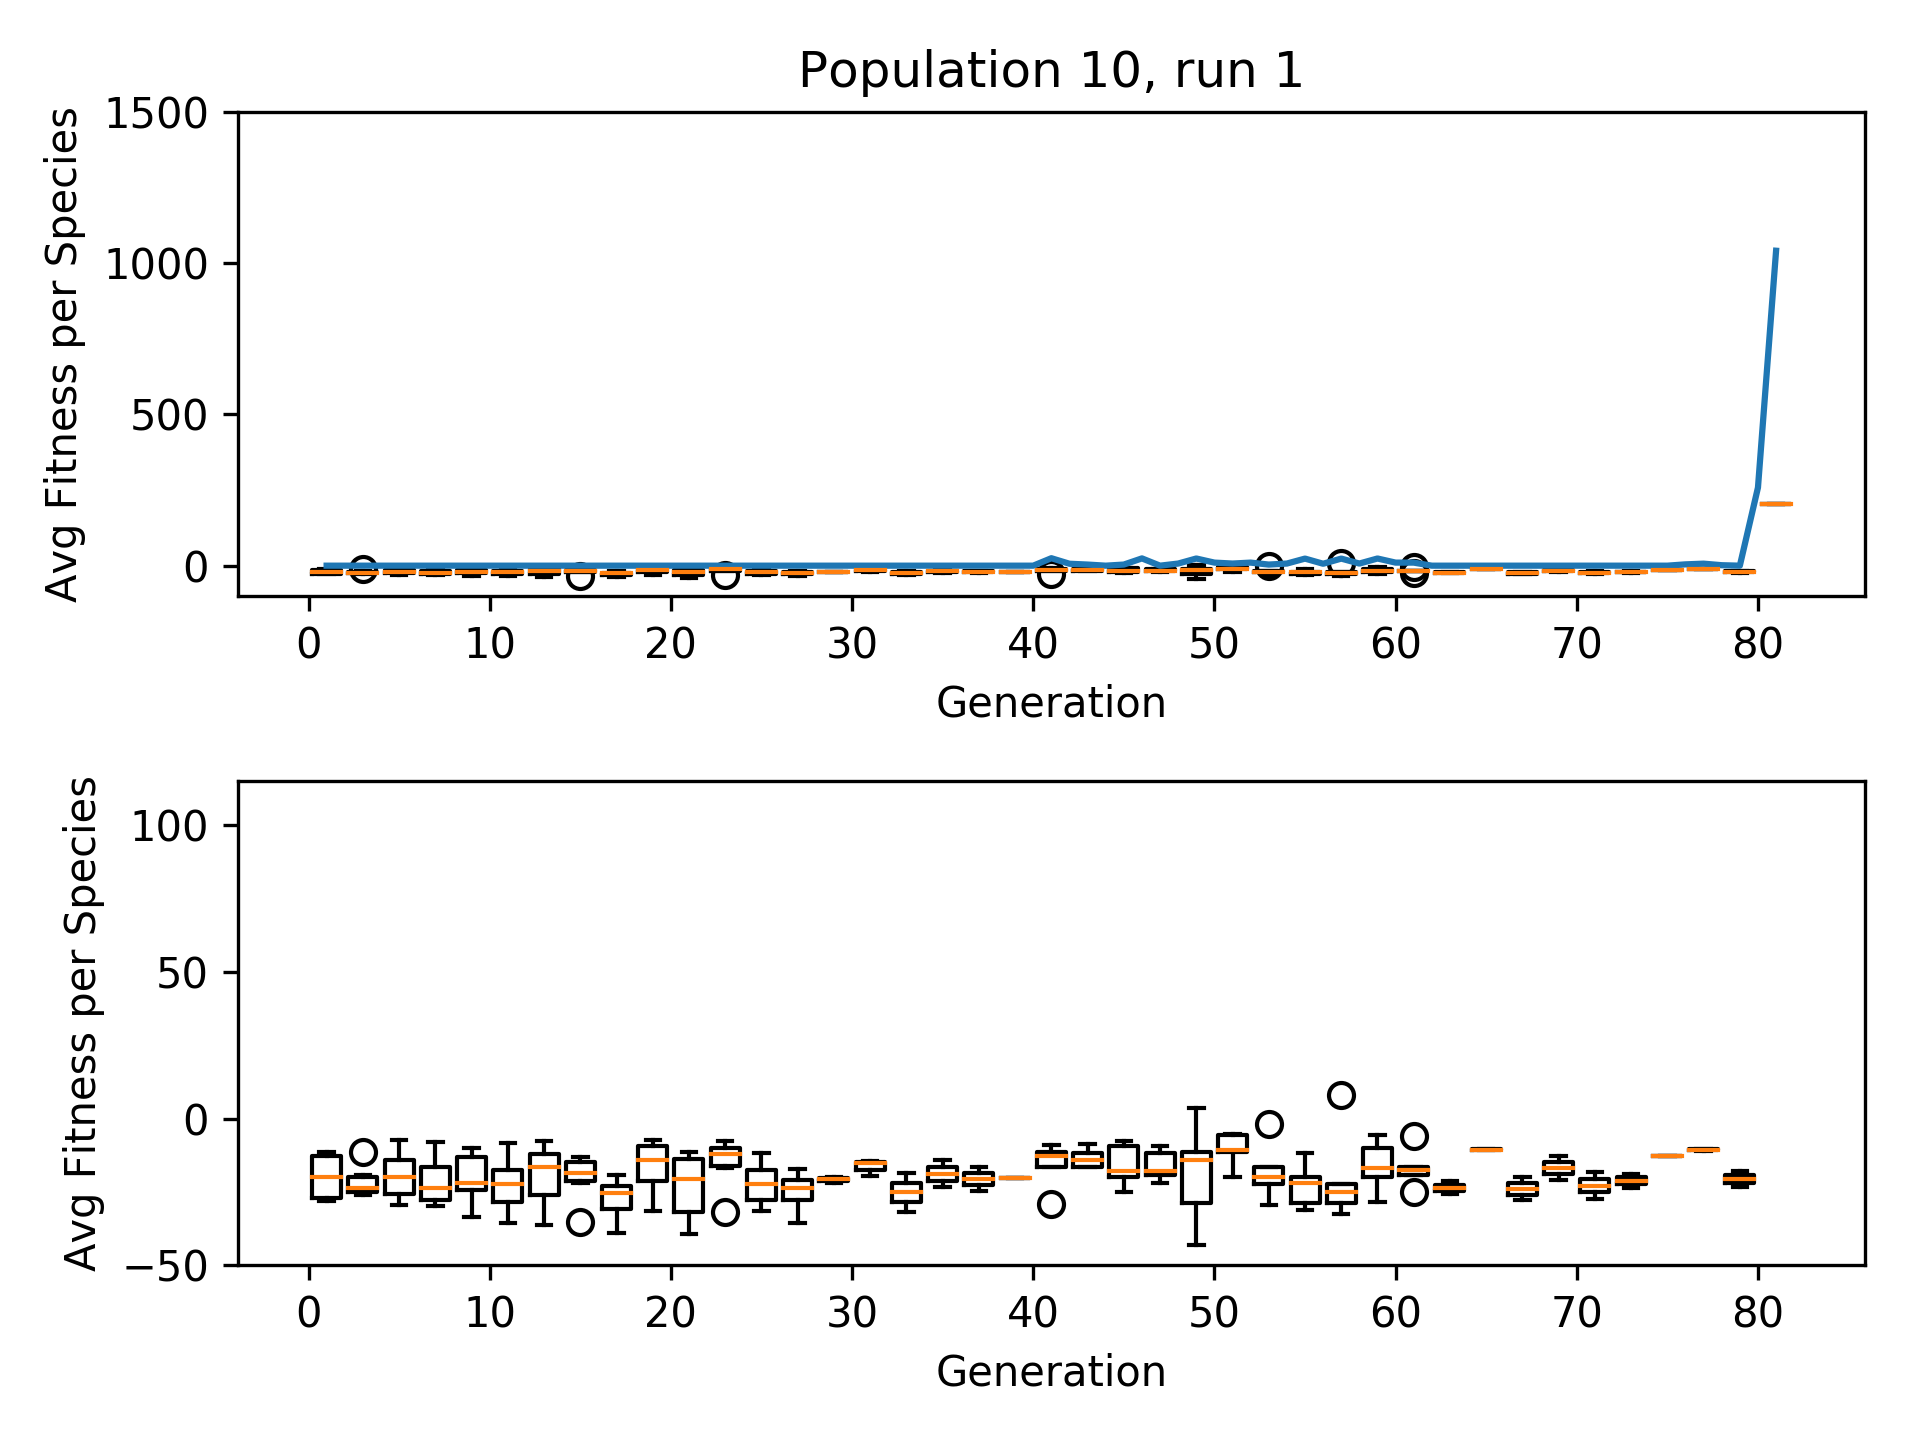
\includegraphics[width=1\textwidth]{graphics/flappy/pop10_run1} % first figure itself
				\end{minipage}\hfill
				\begin{minipage}{0.33\textwidth}
					\centering
					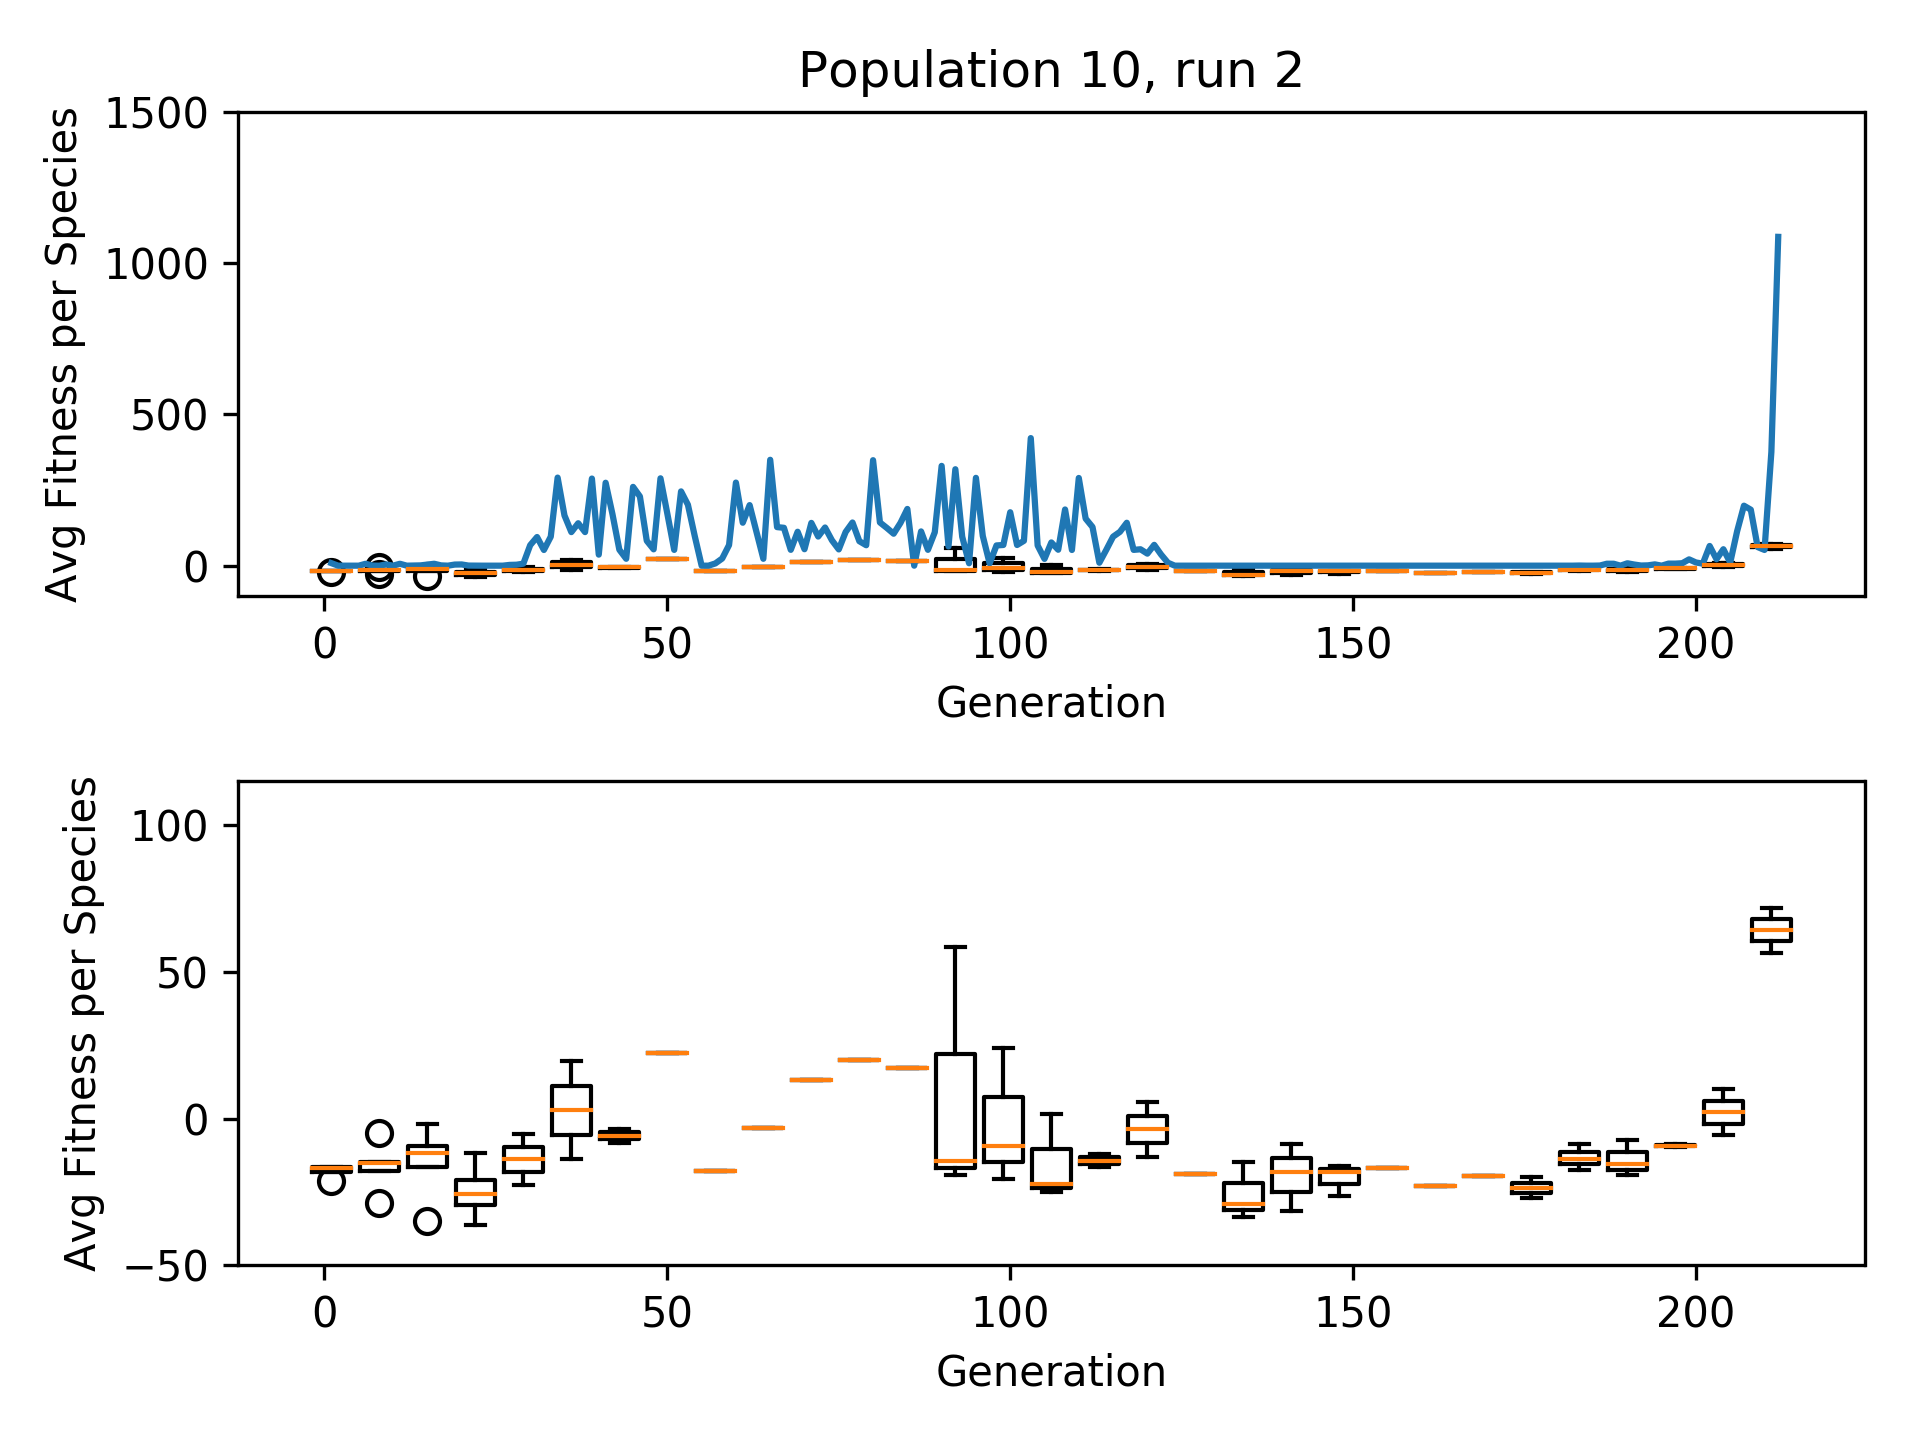
\includegraphics[width=1\textwidth]{graphics/flappy/pop10_run2} % second figure itself
				\end{minipage}
				\begin{minipage}{0.33\textwidth}
					\centering
					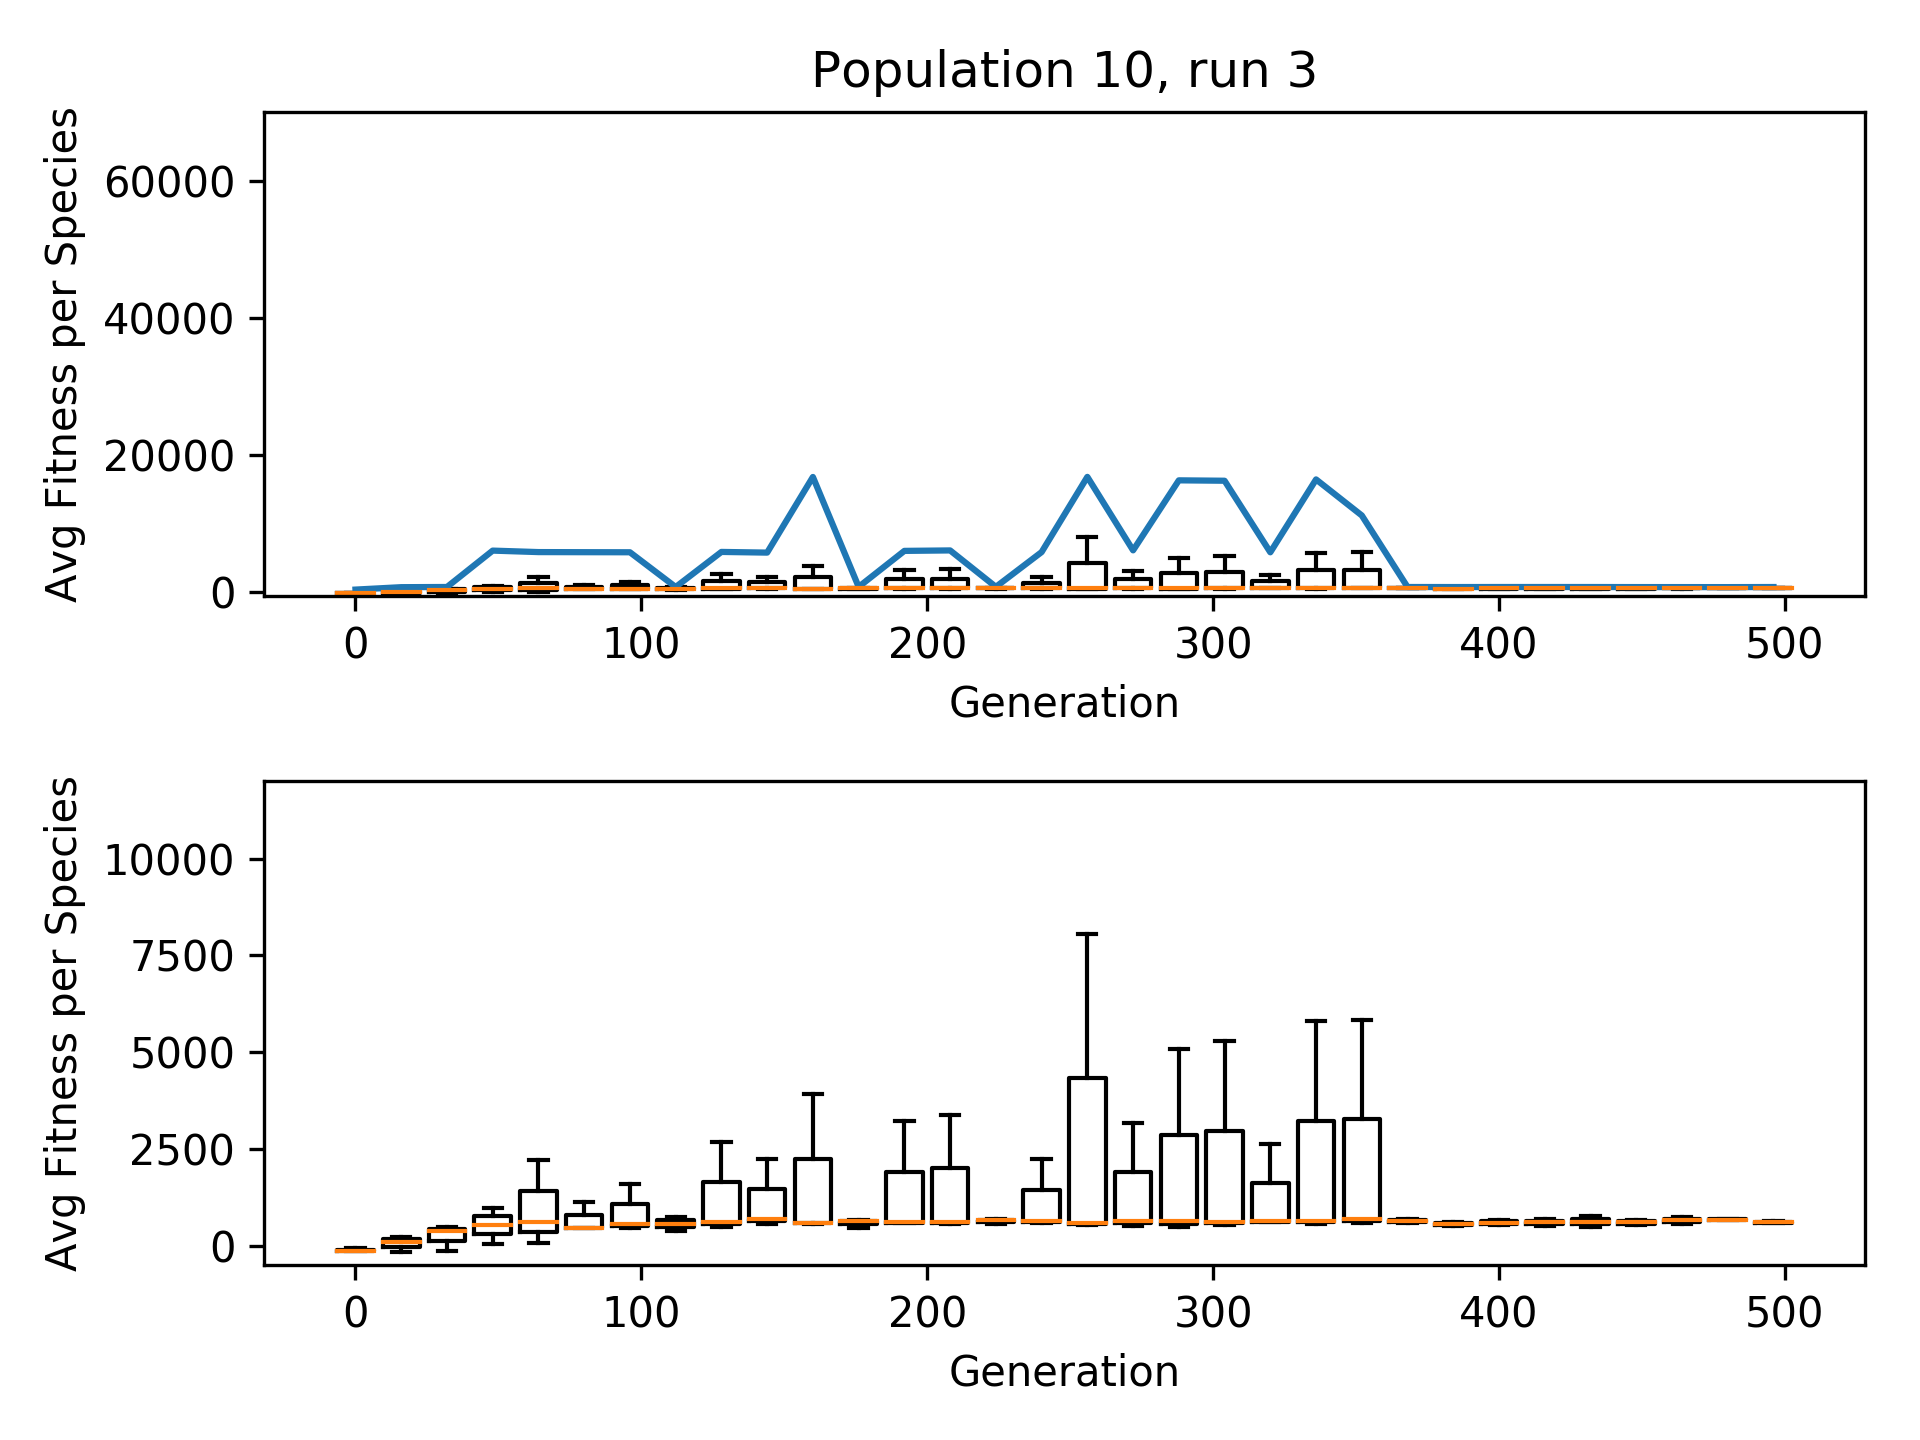
\includegraphics[width=1\textwidth]{graphics/flappy/pop10_run3} % second figure itself
				\end{minipage}
				\caption{Flappy Bird Population 10}
				\label{fig:flappy10}
			\end{figure}
			As it is with the graphical representations of MarI/O (see figure \ref{fig:mario10} for example) the vertical axis shows the fitness score average of the genomes within a species. Again, the horizontal axis portrays the generations containing the species. Each generation contains up to 10 populations which are divided into species and genomes within species. In this \gls{neat}-implementation a fixed size of generations was specified.\\
			As in MarI/O the best runs of genomes per generation is marked with a blue line. In the Flappy Bird simulations the best runs and the median of each species (or the $average\_distance$ described in section \ref{par:mario10}) are to far apart to be able to display them in one graph of linear scale. That's why two graphs are shown with different fitness ranges. The upper part displays a range from -100 to 1500 and the upper plot shows values in the range of -50 to 115 fitness score.\\
			Although the $average\_distance$  is big in general, this plot-run has the smallest $avergage\_distance$ of the three simulation classes with an average value of $51.3$.
			In this three plot-runs the upper boundary was $500$ generations, however, there was an fitness-threshold implemented as well which ended the simulation when a fitness score over 600 was reached. Plot-run 1 launched 81 generations, plot-run 2 launched 307 generations and plot-run 3 had 367 generations before this threshold was exceeded. This results in an average skipping of $8.3\overline{8}$ generations inside the graphs, between two displayed generations. \\
			Interestingly, plot-run 2 and 3 managed to enhance their score by generation 30 but dropped again latest at generation 130, however, all three plot-runs managed to reach a score beyond 600. Plot-run 1 reached this goal the earliest in generation 81 and therefore needed less than a third of the generations plot-run 2 and 3 spawned.\\
			In comparison to MarI/O (see section \ref{sec:analysis:mario}) wherein generation 0 there were as many species spawned as configured with the population size, whereas every species contained only 1 genome, this implementation of the \gls{neat} algorithm spawns the configured amount of genomes first and after the first simulation run assigns them into species. Moreover, the generation number starts from 1 and not from 0 as in MarI/O. So after the first run on average $5.\overline{3}$ species where classified. In generation 80 on average $1.\overline{6}$ species where left. Since there was a setting configured which reset the species if a total extinction (no species left) has occurred. These values have to be considered carefully.\\
			In plot-run 2 and 3 there was a significant $average\_regress$ made of approximately $-24.54$ in plot-run 2 and $-11.38$ in plot-run 3. Plot-run 2 regressed 67 times and plot-run 3 41 times. Plot-run 1 kept the $average\_regress$ far lower with an approximate value of $-1.42$.\\
			Since plot-run 1 has the fewest generations the $average\_fitness\_increase$ is the highest with a value of around $16.04$, whereas plot-run 2 has a value of $\approx6.86$ and plot-run 3 of $\approx10.54$. However, the average score of each generation is the lowest in plot-run 1 ($\approx-15.87$). Plot-run 2 has a value of about $-4.22$ and plot-run 3 of $-10.62$. \\
			Since the game environment is open-ended the expectations from MarI/O (see \ref{par:mario10}) that $\lim\limits_{n \to \infty} average\_fitness\_increase(n) = 0$ does not hold here. However, the opposite is true that $\lim\limits_{n \to \infty} average\_fitness\_increase(n) = \infty$ is to be expected. Therefore there was the fitness-threshold introduced to end the simulation before an infinite flight is expected.
		
		\paragraph{Population 50 / Generation 100}
			\begin{figure}[h]
				\centering
				\begin{minipage}{0.33\textwidth}
					\centering
					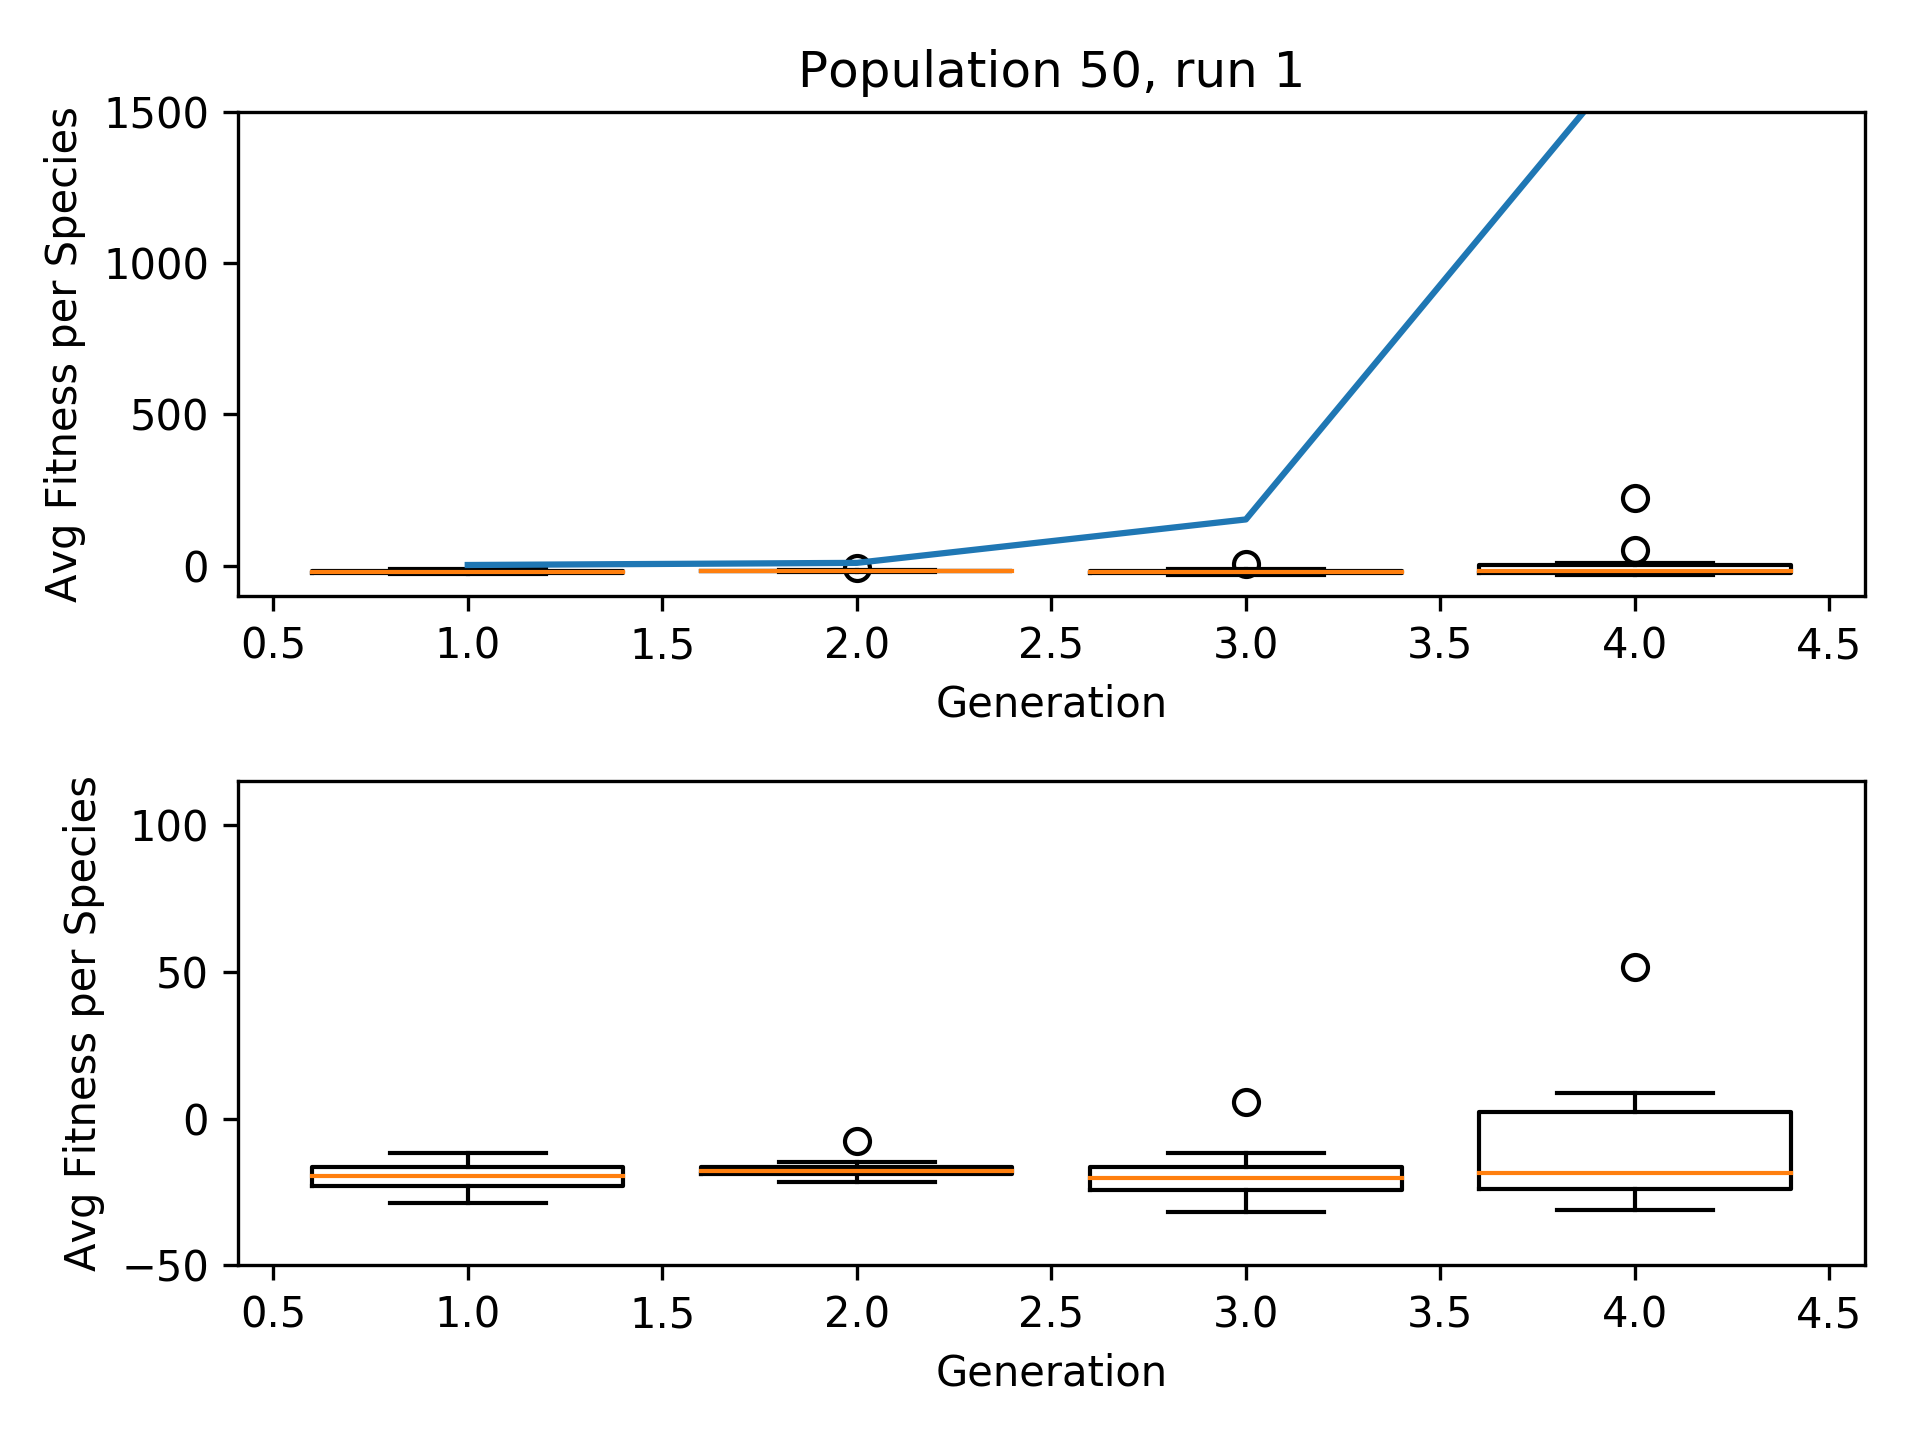
\includegraphics[width=1\textwidth]{graphics/flappy/pop50_run1} % first figure itself
				\end{minipage}\hfill
				\begin{minipage}{0.33\textwidth}
					\centering
					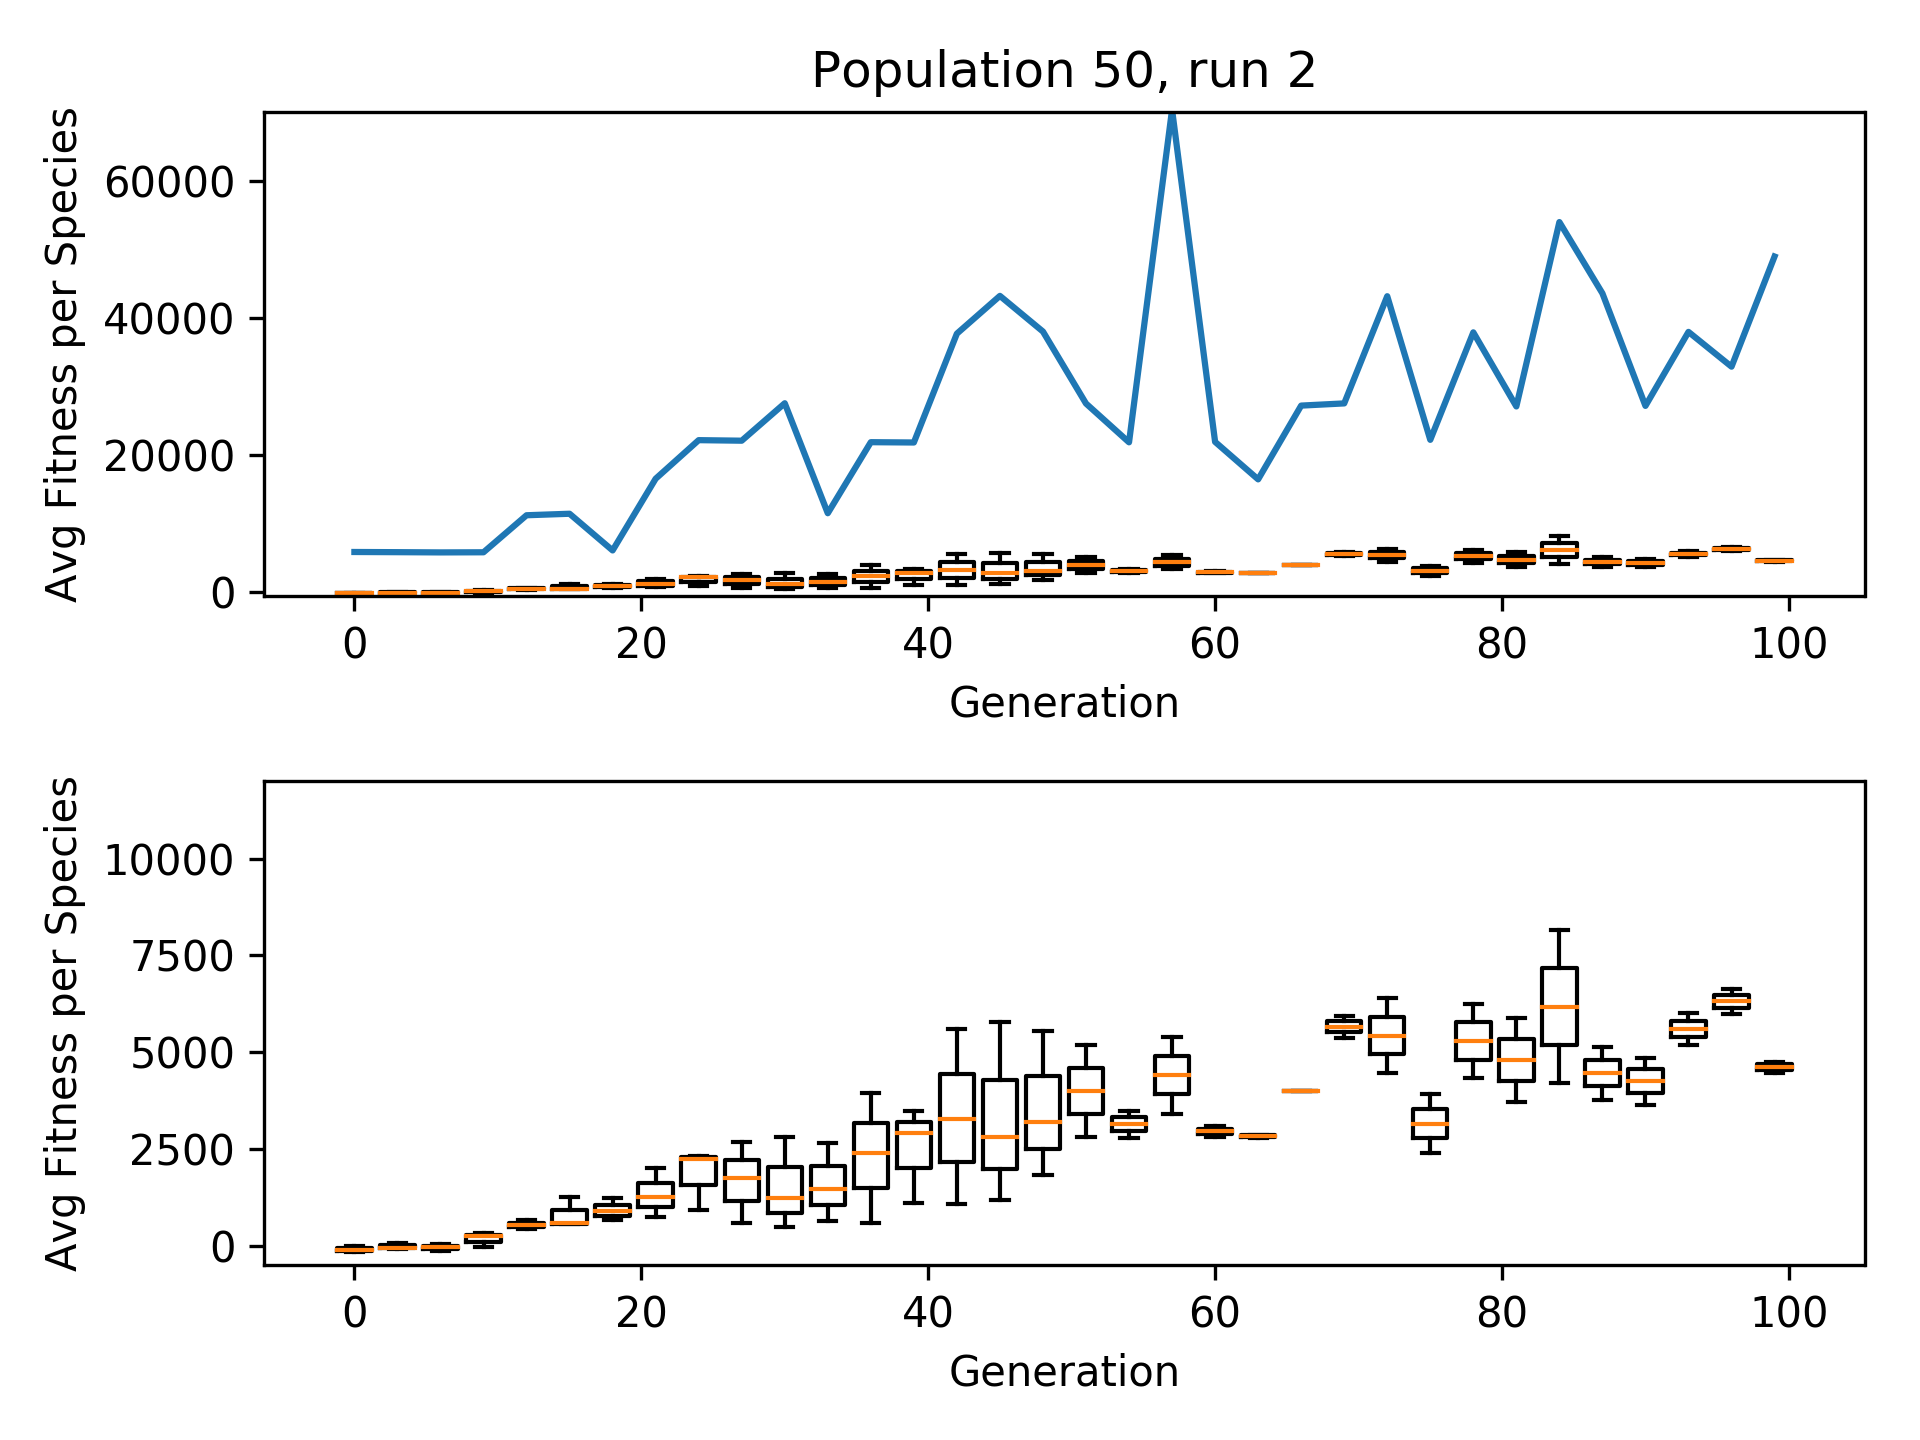
\includegraphics[width=1\textwidth]{graphics/flappy/pop50_run2} % second figure itself
				\end{minipage}
				\begin{minipage}{0.33\textwidth}
					\centering
					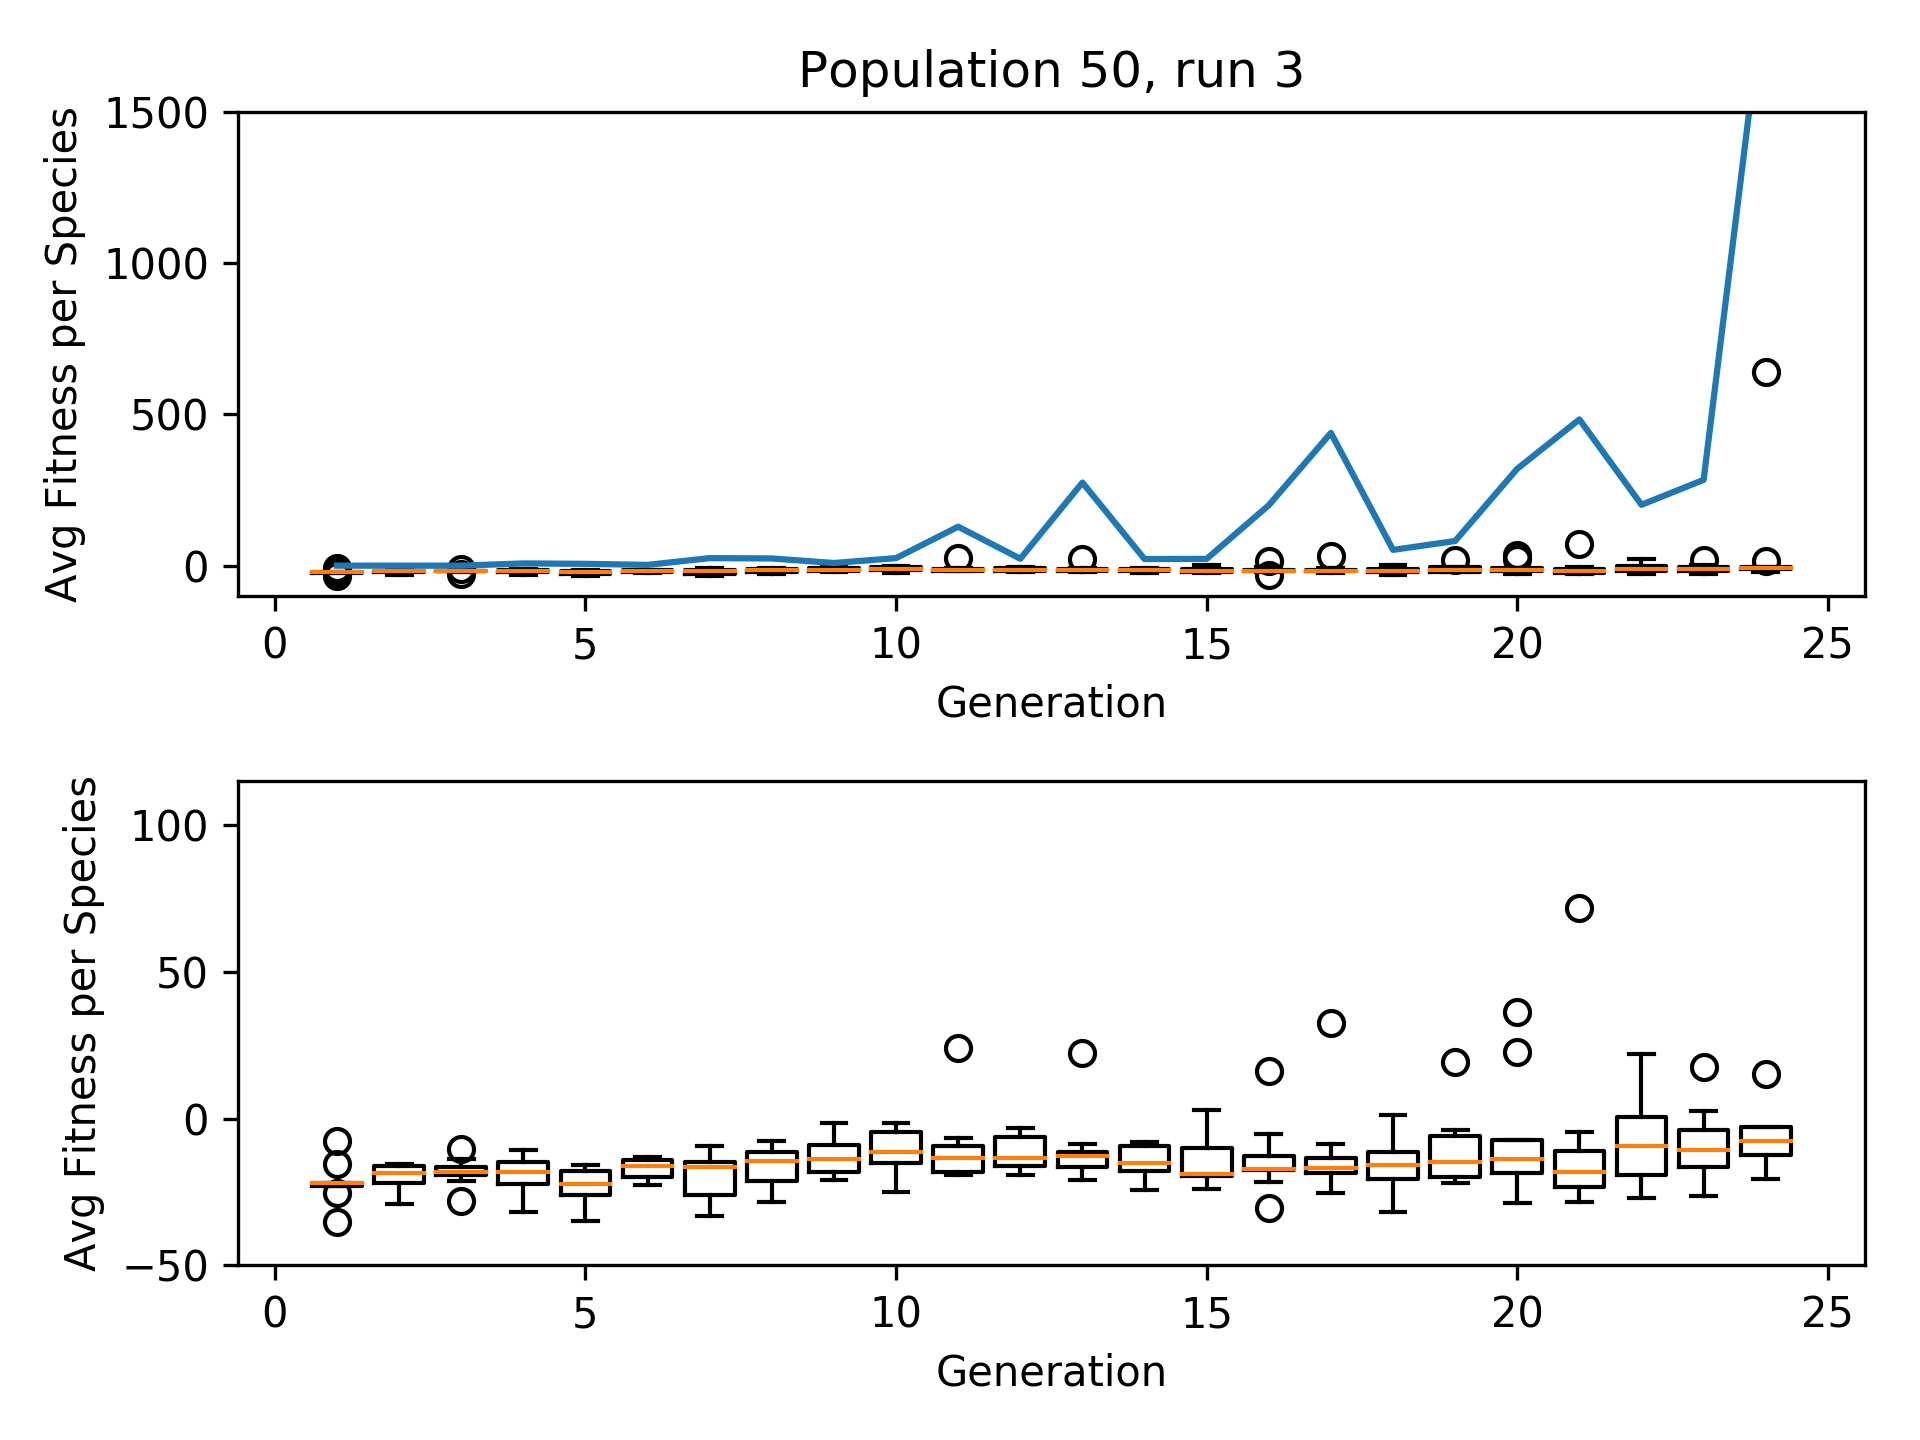
\includegraphics[width=1\textwidth]{graphics/flappy/pop50_run3} % second figure itself
				\end{minipage}
				\caption{Flappy Bird Population 50}
				\label{fig:flappy50}
			\end{figure}
			These simulations have an average $average\_distance$ of $270.25$. In this instance, the standard deviation should be taken into account, which is also quite high with a value of 192.24. 
			In the plot-runs of this population class, the upper boundary was $100$ generations, however, again the fitness-threshold of 600 was exceeded in every plot-run. Plot-run 1 launched 4 generations, plot-run 2 launched 9 generations and plot-run 3 had 24 generations when the threshold was exceeded. Therefore no generation had to be skipped in the graphical display.\\
			After the first run, in generation 1, the genomes were divided into $9.\overline{3}$ species on average. At the end of generation 4, plot-run 2 and 3 kept their species and plot-run 1 lost one species. The species-reset did not had to be used at this point. In plot-run 3, 7 species were left at the end (generation 24).
			In plot-run 1 no regress occurred and in plot-run 2 only one time a regress was made which results in an average-regress of $-0.07$. Plot-run 3 had many potential outbreaks which resulted in 9 regresses with an $average\_regress$ of $\approx-45.84$.\\
			The $average\_fitness\_increase$ is the highest in plot-run 1 since the generation count is the smallest. Its value is $461.52$. The $average\_fitness\_increase$ values are similar in plot-run 2 and 3 with approximately 87.93 in plot-run 2 and 92.79 in plot-run 3. The average score of each generation remains negative in this simulations for all plot-runs.
		
		\paragraph{Population 250 / Generation 30}	
			\begin{figure}[h]
				\centering
				\begin{minipage}{0.33\textwidth}
					\centering
					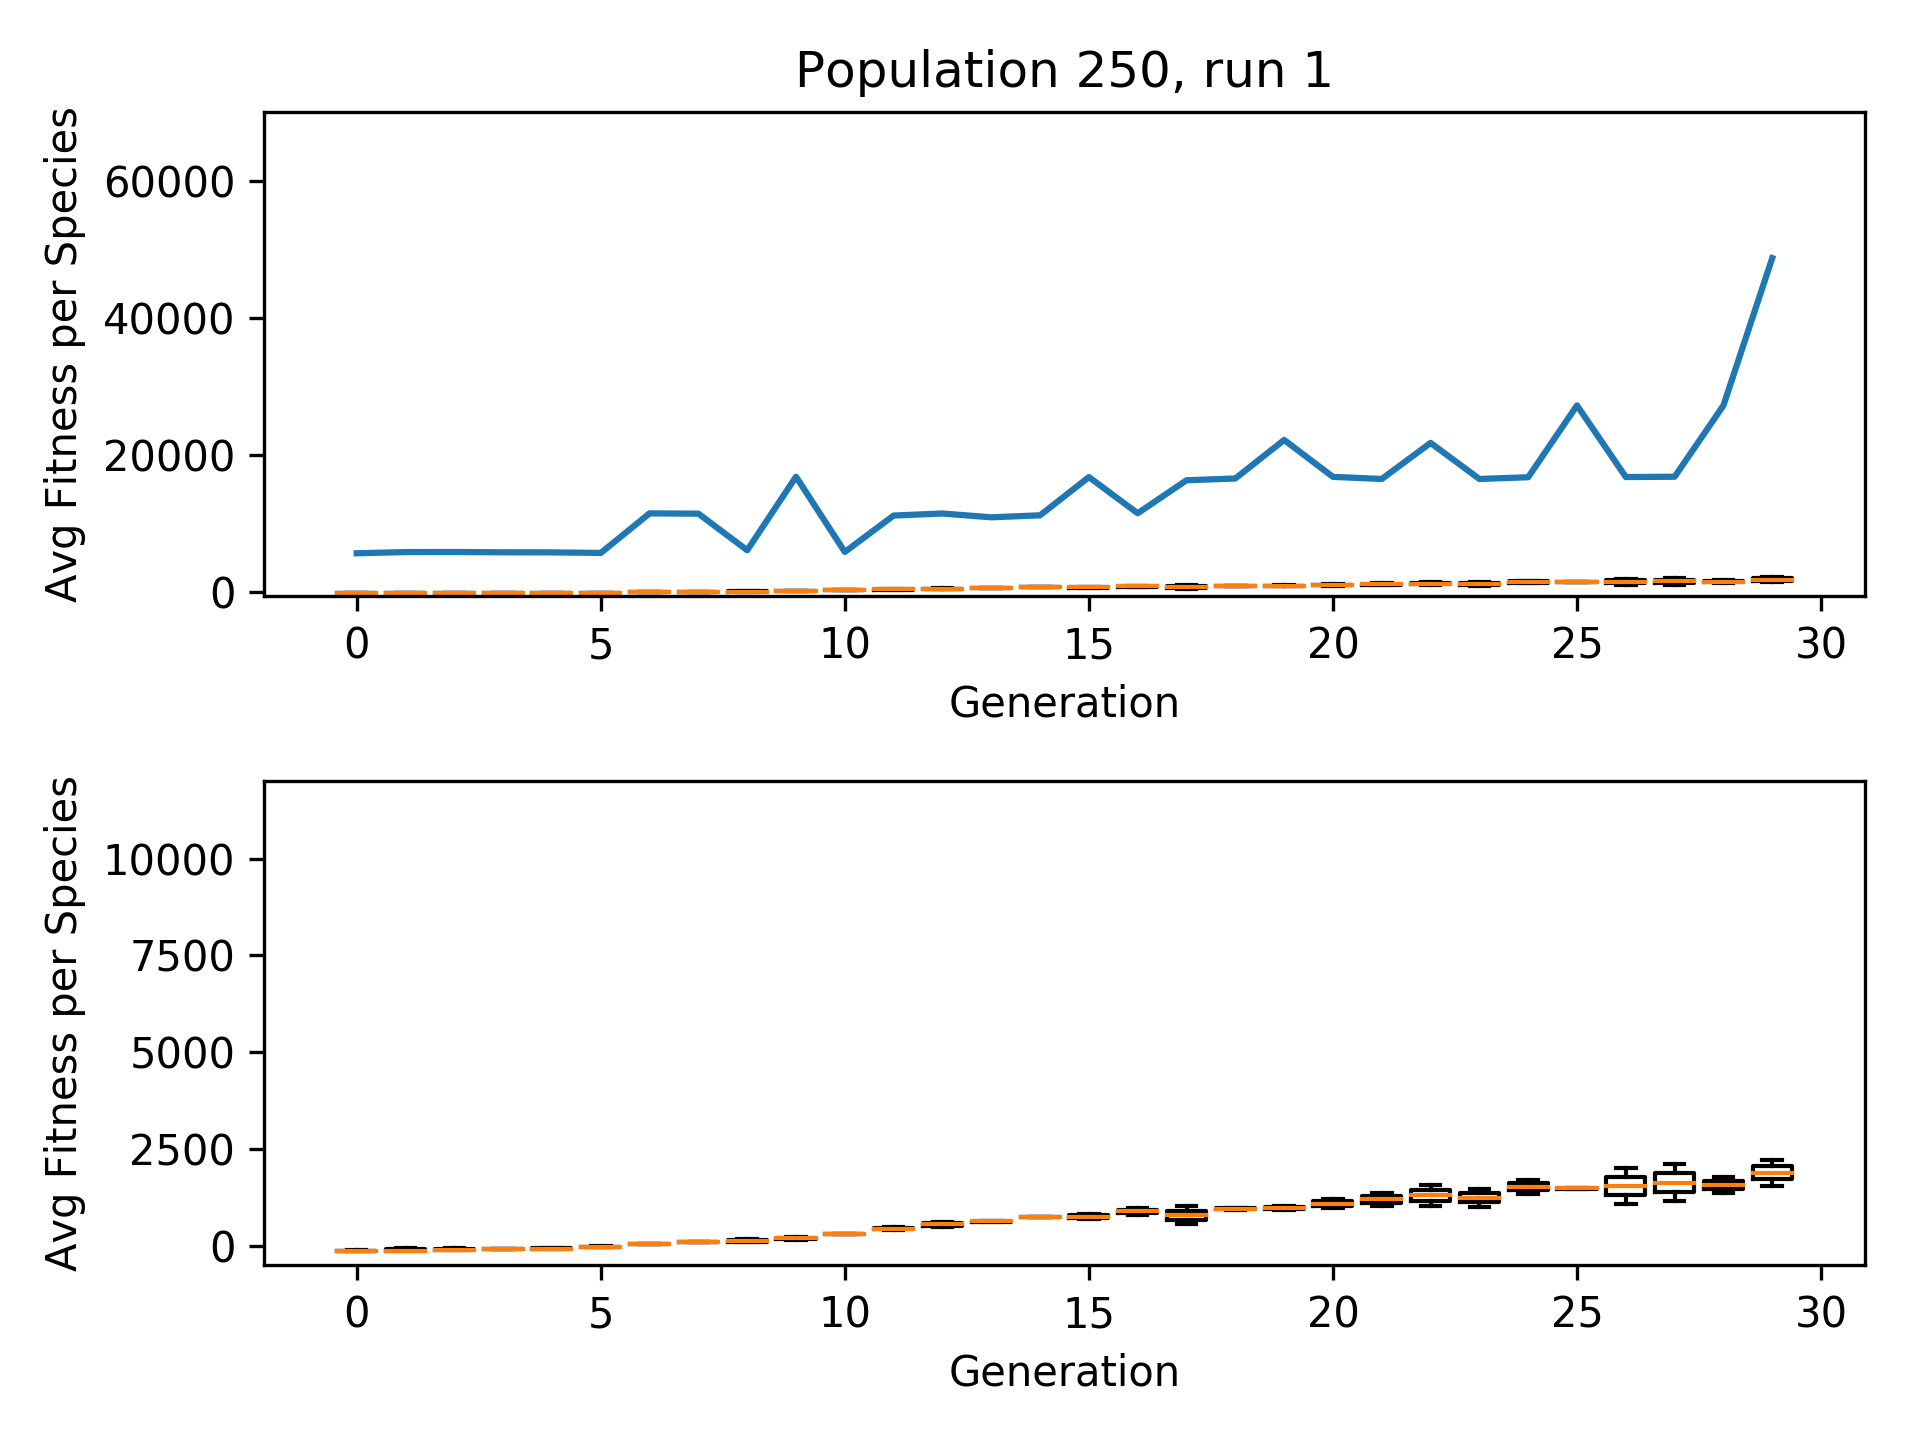
\includegraphics[width=1\textwidth]{graphics/flappy/pop250_run1} % first figure itself
				\end{minipage}\hfill
				\begin{minipage}{0.33\textwidth}
					\centering
					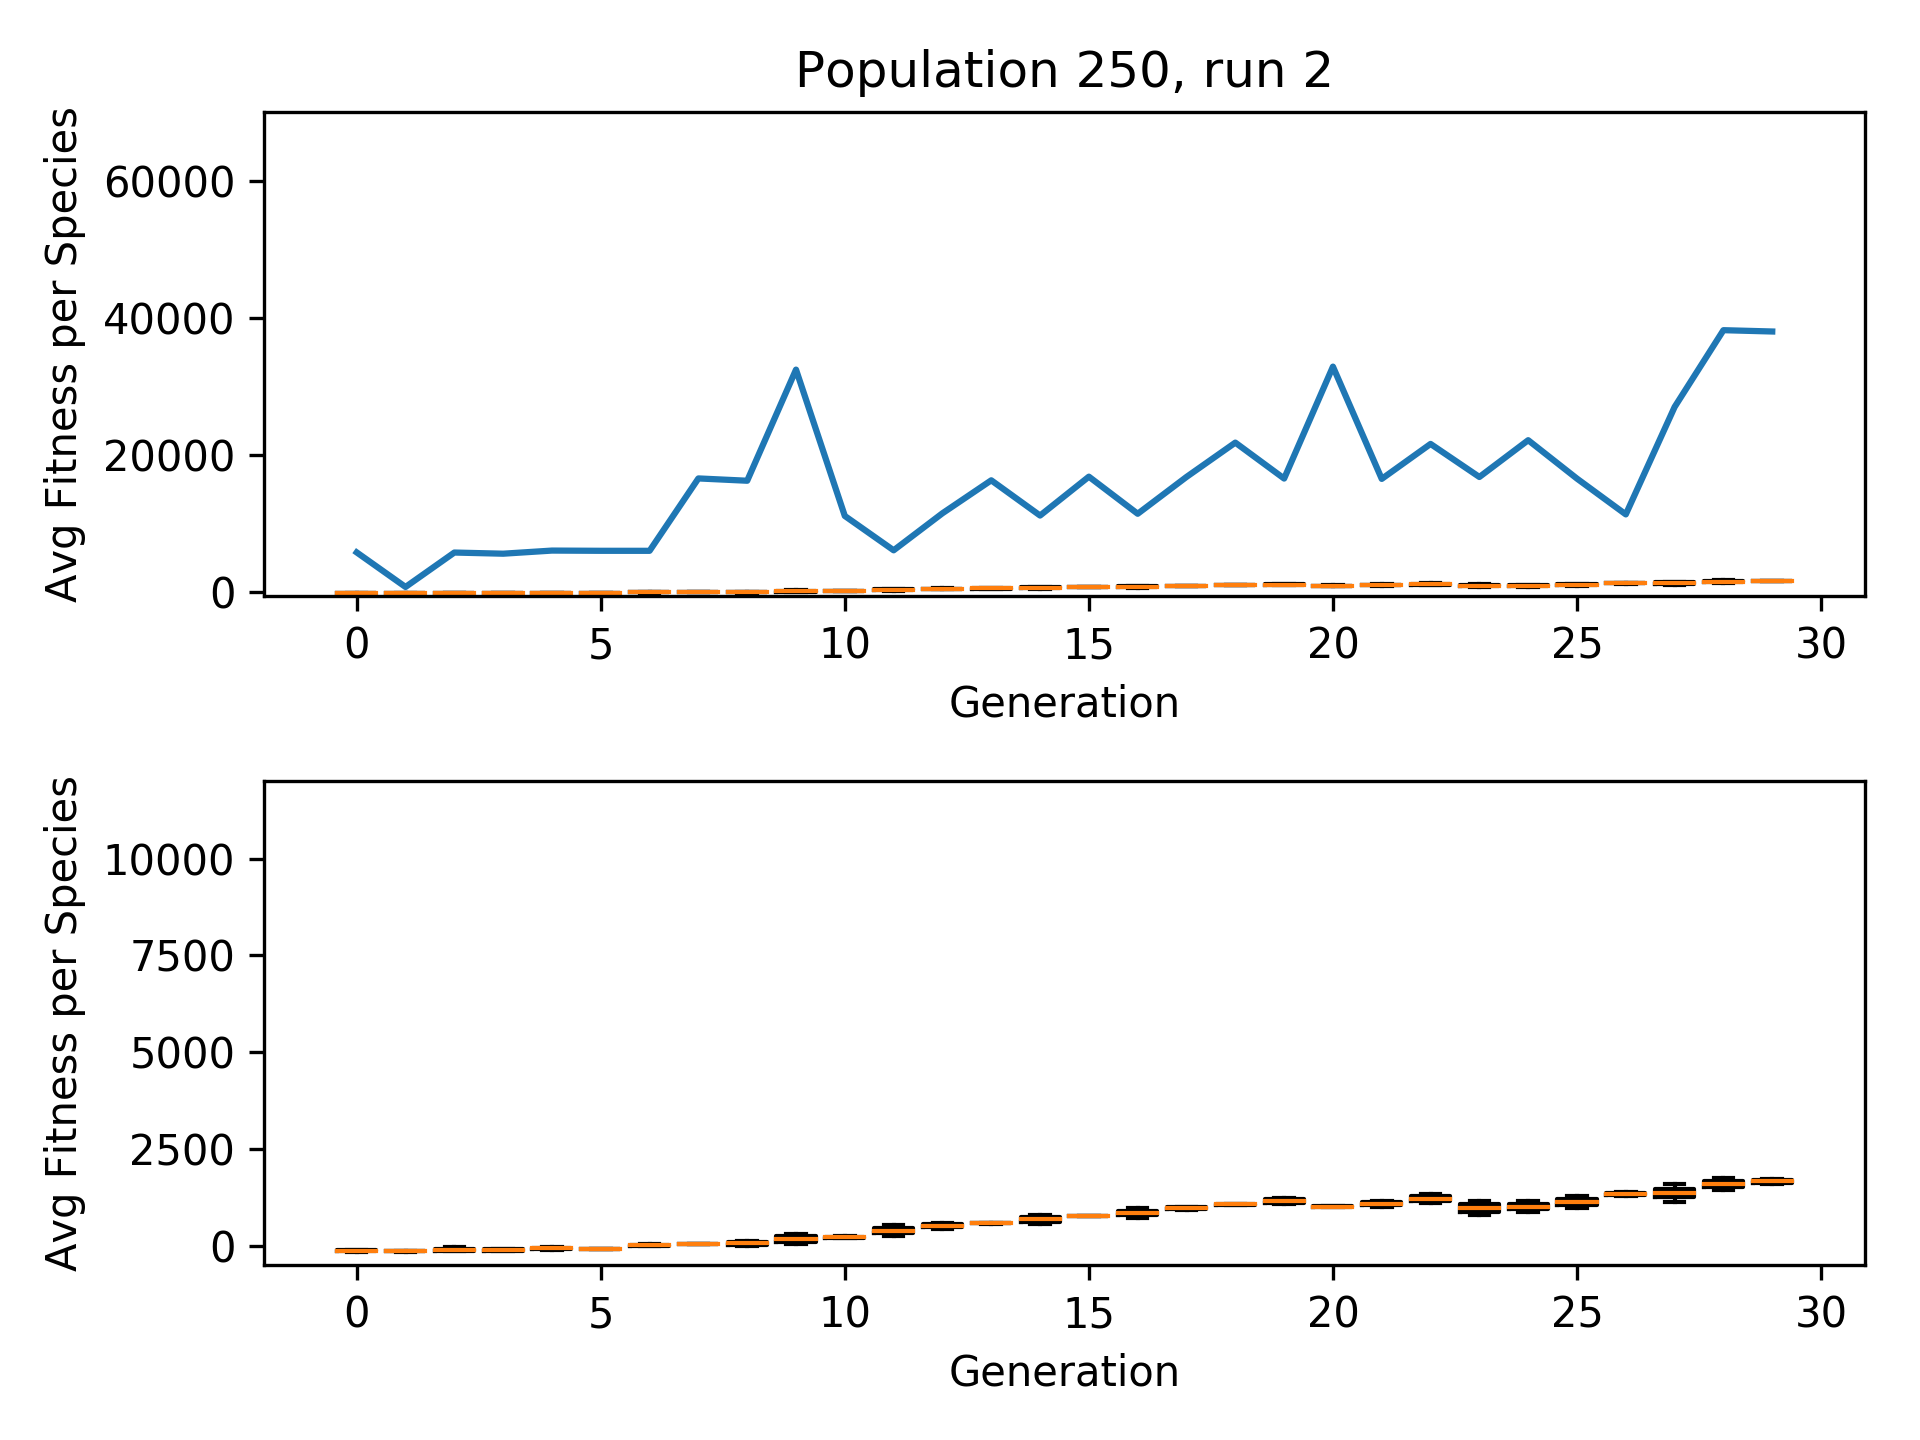
\includegraphics[width=1\textwidth]{graphics/flappy/pop250_run2} % second figure itself
				\end{minipage}
				\begin{minipage}{0.33\textwidth}
					\centering
					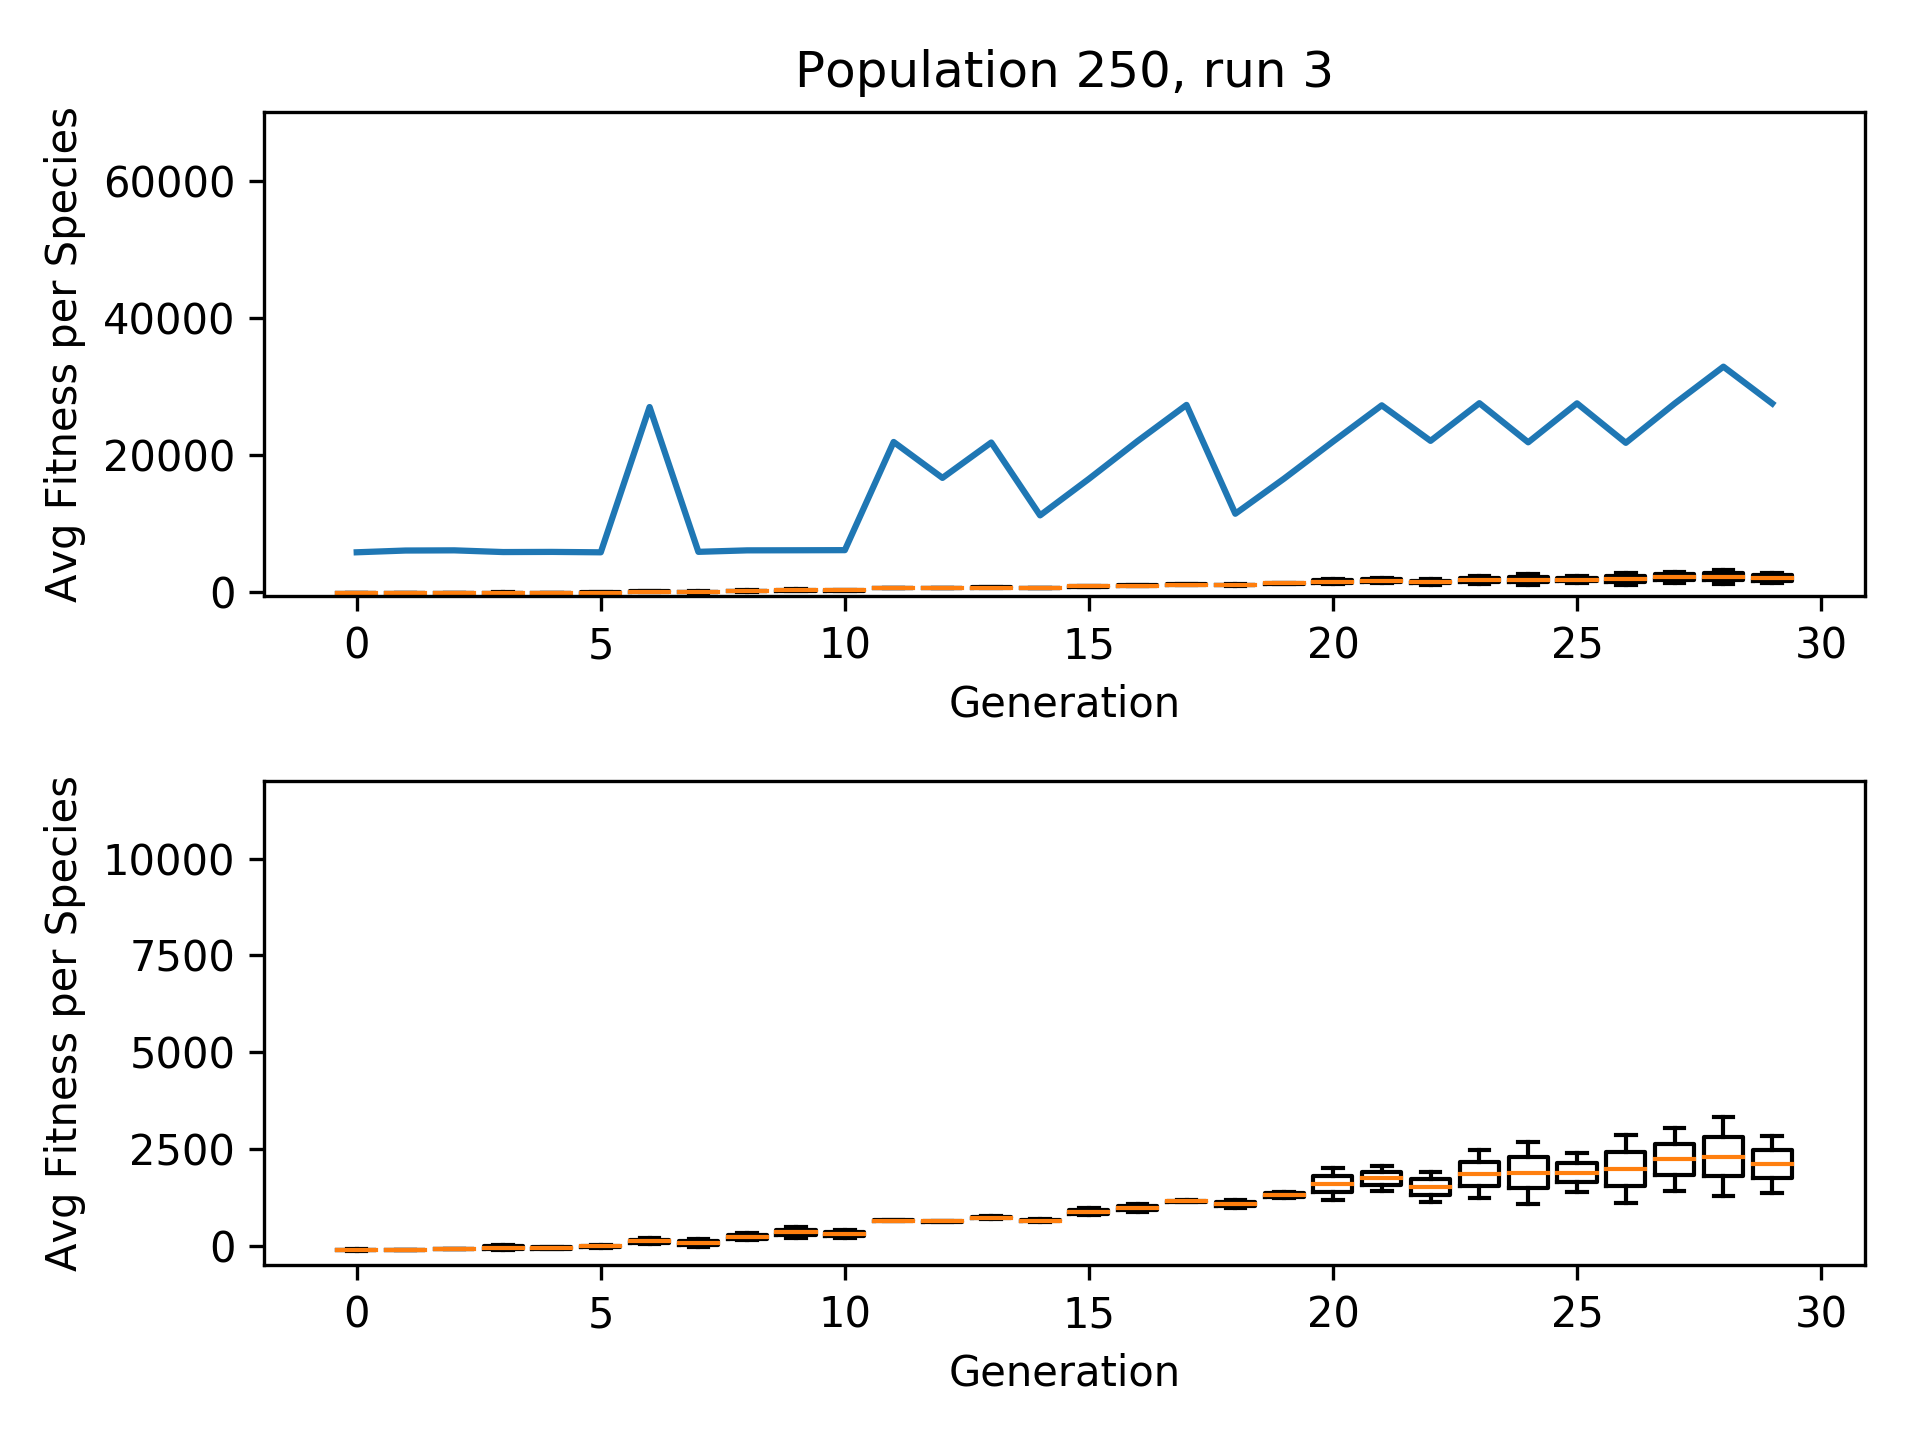
\includegraphics[width=1\textwidth]{graphics/flappy/pop250_run3} % second figure itself
				\end{minipage}
				\caption{Flappy Bird Population 250}
				\label{fig:flappy250}
			\end{figure}
			In three plot-runs have an average $average\_distance$ of $636.5$. Compared to the population 50 instances the standard deviation is lower with a value of $\approx63.14$. 
			In the plot-runs of this population class, the upper boundary was $30$ generations, however, again the fitness-threshold of 600 was exceeded in every plot-run. Plot-run 1 and 2 launched 3 generations, and plot-run 3 had 4 generations when the threshold was exceeded. Again, no generation had to be skipped in the graphical display.\\
			After the first run, in generation 1, the genomes were divided into $22.\overline{3}$ species on average. At the end of generation 3, all plot-runs contained more than 10 species each.\\
			Interestingly all plot-runs could avoid regress within the next generations. \\
			The $average\_fitness\_increase$ was high in general with a value of 433.86 in plot-run 1, 537.57 in plot-run 2 and 347.07 in plot-run 3 since there were few generations spawned.\\
			Since the \gls{neat} algorithm had no problems with this game it is more interesting to see how this population classes compare to one another.
		
		\paragraph{Comparison of the results}
			\begin{table}[h]
				\centering
				\resizebox{\textwidth}{!}{
					\begin{tabular}[width=0.5\textwidth]{@{}ll|l|l|l|l@{}}
						\toprule
						{\Large NEAT\_FlappyBird} 	& avg. runs /$\sigma$ 			& avg. fitness score /$\sigma$ 	& avg distance /$\sigma$ 	& avg. regress /$\sigma$ 	& avg. fitness increase /$\sigma$ 	\\ \midrule
						Population 10  				& 1684 /714.01             		& -10.23 /5.84      			& 51.3 /18.93         		& -12.45 /11.59      		& 11.15 /4.62            			\\
						Population 50  				& $626.\overline{6}$ /531.71	& -9.77 /2.95       			& 270.24 /192.24        	& -15.30 /26.45      		& 214.08 /214.30           			\\
						Population 250 				& $831.\overline{6}$ /139.72 	& -13.81 /1.38       			& 638.5 /63.14        		& 0 /0     					& 439.5 /95.38         				\\ \bottomrule
					\end{tabular}
				}
				\caption{Flappy Bird Population Comparison Overview}
				\label{tab:flappy}
			\end{table}
	
			\todo{Differences and similarities between runs in graph} \\
			In order to compare the results, the same 5 distinct values (see table \ref{tab:flappy}) of the plot-runs where calculated, which were taken into consideration in section \ref{sec:analysis:mario}.\\
			The most obvious observation is that the average fitness increase rises with the number of populations used since the generations remain low in the count when the threshold is reached. Secondly, the average distance (from the species median to the best genome run) tend to rise as well with a bigger population size.\\ 
			The other measurement values leave little to no conclusions since the values don't rise or fall with growing/shrinking population sizes. The average regress, for example, tends to rise between population class 10 and 50 but is 0 in population class 250. The question is if the population class 250 would have a greater regress than the other two population instances if there would be any (future) regress. The average fitness score is non-rising/shrinking as well, however, the standard deviation seems to shrink with greater population size. Probably, the negative values of the fitness score depend on the environment of Flappy Birds, where only partially well-learned birds can make it through the first obstacle (namely the pipes).\\
			Since there is no defined goal, the fitness-threshold can be taken into consideration when deciding how good simulations have been. Since the threshold was exceeded in every plot-run, the last generation holds the best run of a plot-run. The fewest average runs were done by population class 50 with averaged $626.\overline{6}$ runs. However, population class 250 had the smallest standard deviation of their running length, which indicates that the goal can be more consistently reached around the $831.\overline{6}$th run compared to population count 10 and 50.
			
		\subsection{Plain Machine learning flappy bird}
			\begin{enumerate}
				\item better results
				\item multi simulation made it easier
				\item easy algorithm for easy environment might be explanation for better results
				\item \begin{enumerate}
					\item Differences between runs (lucky runs with 4th champion generation)
				\end{enumerate}
			\end{enumerate}
			\paragraph{Comparison to \gls{neat} results}